% Chapter 3:

\chapter{High-Level Programming for Multi-GPU Systems}

\label{chapter:skelcl}

In this chapter we address the first main challenge identified in \autoref{chapter:background}: Programmability.
We will see how structured parallel programming simplifies the task of programming for parallel systems.
As throughout the thesis, we will focus on programming of single- and multi-\GPU systems.
We will first motivate the need for high-level abstractions using an real-world \OpenCL application.
Then we introduce the \emph{\SkelCL} programming model and its implementation as a \Cpp library which addresses the lack of high-level abstractions in state of the art \GPU programming models.
The following \autoref{chapter:skelcl-evaluation} will provide several application studies to thoroughly evaluate the usefulness and performance of the abstractions and implementation presented in this chapter.


% ============================================================================ %
\section{The need for high-level abstractions}
\label{section:opencl-example}

\subsection{Requirements to a High-Level Programming Mode}
\label{section:requirements}
The described implementation of the example application reveals the main problems and difficulties that the application developer has to overcome when using \OpenCL.
Our analysis show that to simplify programming for a system with multiple \GPUs, at least the following three high-level abstraction are desirable:

\paragraph{Parallel container data types}
Compute intensive applications typically operate on a (possibly big) set of data items.
As shown in Listing~\ref{lst:upload}, managing memory is error-prone because low-level details, like offset calculations, have to be programmed manually.

A high-level programming model should be able to make collections of data automatically accessible to all processors in a system and it should provide an easy-to-use interface for the application developer.

\paragraph{Recurring patterns of parallelism}
While each application (of course) performs different concrete operations, the general structure of parallelization resembles parallel patterns that are commonly used in many applications.
% In step 1, for computing the error image $c_l$, the same sequence of operations is performed for every event from the input subset, which is the well-known \emph{map} pattern of data-parallel programming~\cite{gc11}.
% In step 2, two images (the current image estimate $f_l$ and the error image $c_l$) are combined element-wise into the output image ($f_{l+1}$), see line 5 of Listing~\ref{lst:step_2}, which is again the common \emph{zip} pattern of parallelism.
It would be, therefore, desirable to express the high-level structure of an application using pre-defined common patterns, rather than describing the parallelism manually in much detail.

\paragraph{Distribution and redistribution mechanisms}
To achieve scalability of applications on systems comprising multiple \GPUs, it is crucial to decide how the application's data are distributed across all available \GPUs.
Distributing and re-distributing data in \OpenCL is cumbersome because data transfers have to be managed manually and performed via the \CPU, as shown in Listing~\ref{lst:redistribution}.
Therefore, it is important for a high-level programming model to allow both for describing the data distribution and for changing the distribution at runtime.


% ============================================================================ %
\section{The SkelCL Programming Model}
\label{section:skelcl-programming-model}
We develop our \SkelCL programming model as an extension of the standard \OpenCL programming model~\cite{OpenCL}.
\SkelCL adds to \OpenCL three features that we identified as desirable in~\autoref{section:requirements}:

\begin{itemize}
  \item \emph{parallel container data types} for unified memory management between host and devices;
  \item \emph{algorithmic skeletons} for easily expressing parallel computation patterns;
  \item \emph{data distribution} and \emph{redistribution} mechanisms for programming multi-device systems.
\end{itemize}

\noindent
\SkelCL inherits all properties of \OpenCL, including its portability across different heterogeneous parallel systems.
\SkelCL is designed to be fully compatible with \OpenCL: arbitrary parts of a \SkelCL code can be written or rewritten in \OpenCL, without influencing program's correctness.


\subsection{Parallel Container Data Types}
\label{section:skelcl-programming-model:container}
\SkelCL offers the application developer two container classes -- vector and matrix -- which are transparently accessible by both, host and devices.
The \emph{vector} abstracts a one-dimensional contiguous memory area while the \emph{matrix} provides an interface to a two-dimensional memory area.
When a container is created on the host, memory is allocated on the devices automatically;
when a container on the host is deleted, the memory allocated on the devices is freed automatically.

The main advantage of the container data types in \SkelCL as compared with \OpenCL is that the necessary data transfers between the host and devices are performed implicitly.
Before performing a computation on container types, the \SkelCL system ensures that all input containers' data is available on all participating devices.
This may result in implicit (automatic) data transfers from the host to device memory, which in \OpenCL would require explicit programming, as we saw in~\autoref{section:opencl-example}.
Similarly, before any data is accessed on the host, the implementation of \SkelCL ensures that this data on the host is up-to-date by performing necessary data transfers implicitly and automatically.
Thus, the container classes shield the programmer from low-level operations like memory allocation (on the devices) and data transfers between host and device.

Developing applications on two-dimensional data for modern parallel architectures is cumbersome and challenging, since efficient memory handling is essential for achieving good performance.
In case of \GPUs, exploiting the memory hierarchy by using the fast but small on-chip memory is key for high performance.
Therefore, in addition to the vector as a one-dimensional abstract data structure, \SkelCL offers a specific abstract data type for handling two-dimensional data, the matrix.

The implementations of the algorithmic skeletons included in \SkelCL differentiate for their input container between vector and matrix, thus, offering optimized implementations for each case.


\subsection{Algorithmic Skeletons}
\label{section:skelcl-programming-model:skeletons}
In original \OpenCL, computations are expressed as \emph{kernels} which are executed in a parallel manner on an \OpenCL device:
the application developer must explicitly the parallelism by specifying how many instances of a kernel are launched in parallel.
In addition, kernels take pointers to device memory as input and contain program code for reading/writing single data items from/to it.
These pointers have to be used carefully, because no boundary checks are performed by \OpenCL.

To shield the application developer from these low-level programming issues, \SkelCL extends \OpenCL by introducing high-level programming patterns, called \emph{algorithmic skeletons}~\cite{Cole1991}.
Formally, a skeleton is a higher-order function that executes one or more user-defined (so-called \emph{customizing}) functions in a pre-defined parallel manner, thus hiding the details of parallelism and communication from the user~\cite{GorlatchCo2011}.

\SkelCL provides four basic data-parallel skeletons: \map, \zip, \reduce, and \scan;
as well as three more specialized skeletons: \mapOverlap, \stencil, and \allpairs.
In this section we will look at the basic skeletons, the specialized skeletons will be discussed later on in this chapter.
The four basic skeletons have been selected, because they are useful for a broad range of applications.
Moreover, these skeletons can be efficiently implemented on \GPUs as their computation patterns match the data-parallel \SIMD (Singe Instruction, Multiple Data) execution model used by \GPUs.

% We define the four basic skeletons using the following notations:
% we use an arrow over lowercase letters to denote vectors, \eg, $\vec{v}$ for a vector of size $n$ with corresponding elements $v_i$ where $0 < i \leq n$.
% We use uppercase letters to denote matrices, \eg, $M$ for an $n\times m$ matrix with corresponding elements $M_{i,j}$ where $0 < i \leq n$ and $0 < j \leq m$.


\paragraph{The \map skeleton}
The \map skeleton is a well known basic algorithmic skeleton, applying a given function to each element of a container.
This skeleton originates from the functional world, where the \code{map} function is recognized as an important primitive for writing high-level code.
In many programming languages an equivalent sequential function exists, either known by the same name, like in Haskell or Python, or by other names, like \code{transform} in \Cpp, or \code{Select} in \Csharp.

In \SkelCL the \map skeleton can operate on vectors as well as matrices.
We start by formally define the skeleton on vectors:
\begin{definition}
  \label{definition:map}
  Let $\vec{x}$ be a vector of size $n$ with elements $x_i$ where $0 < i \leq n$.
  Let $f$ be a unary customizing function.
  The algorithmic skeleton \map is defined as follows:
  \begin{equation}
    map \big(\ f,\ [x_1, x_2, \dots, x_n]\ \big) = [f(x_1), f(x_2), \dots, f(x_n)]
  \end{equation}
\end{definition}
\noindent
The definition for matrices is similar:
\begin{definition}
  \label{definition:map:matrix}
  Let $M$ be an $n\times m$ matrix with elements $M_{i,j}$ where $0 < i \leq n$ and $0 < j \leq m$.
  Let $f$ be a unary customizing function.
  The algorithmic skeleton \map is defined as follows:
  \begin{equation}
    map\big(\ f,\ \DottedMatrix{M_{0,0}}{M_{0,m}}{M_{n,0}}{M_{n,m}} \big)
      = \DottedMatrix{f(M_{0,0})}{f(M_{0,m})}{f(M_{n,0})}{f(M_{n,m})}
  \end{equation}
\end{definition}
\noindent
The output container, either vector or matrix, can be computed in parallel, because the computation of each single element is independent of each other.

A simple possible application of the \map skeleton is negating all the values in a vector:
\begin{align*}
  neg(\vec{x}) &= map(\ -, \vec{x}\ )
\end{align*}


\paragraph{The \zip skeleton}
The \zip skeleton operates on two containers and combines them in one.
As the \map skeleton it is defined for vectors and matrices as well.
\begin{definition}
  \label{definition:zip}
  Let $\vec{x}$ and $\vec{y}$ be vectors of size $n$ with elements $x_i$ and $y_i$ where $0 < i \leq n$.
  Let $\oplus$ be a binary customizing operator.
  The algorithmic skeleton \zip is defined as follows:
  \begin{equation}
    \begin{split}
    zip \big(\ \oplus,\ [x_1, x_2, \dots, x_n],\ [y_1, y_2, \dots, y_n]\ \big)\\
      = [x_1 \oplus y_1, x_2 \oplus y_2, \dots, x_n \oplus y_n]
    \end{split}
  \end{equation}
\end{definition}
\noindent
Again the definition for matrices is similar:
\begin{definition}
  \label{definition:zip:matrix}
  Let $A$ and $B$ be $n\times m$ matrices with elements $A_{i,j}$ and $B_{i,j}$ where $0 < i \leq n$ and $0 < j \leq m$.
  Let $\oplus$ be a binary customizing operator.
  The algorithmic skeleton \zip is defined as follows:
  \begin{equation}
    \begin{split}
    zip\big( f,\ {\DottedMatrix{A_{0,0}}{A_{0,m}}{A_{n,0}}{A_{n,m}}},\
                 {\DottedMatrix{B_{0,0}}{B_{0,m}}{B_{n,0}}{B_{n,m}}}\big) \\
      = \DottedMatrix{A_{0,0} \oplus B_{0,0}}{A_{0,m} \oplus B_{0,m}}{A_{n,0} \oplus B_{n,0}}{A_{n,m} \oplus B_{n,m}}
    \end{split}
  \end{equation}
\end{definition}
\noindent
This definitions require the two input containers to be of exactly the same size.
The \zip skeleton is parallelizeable in the same manner as \map, as each element of the output container can be computed in parallel.

A possible application of the \zip skeleton is adding two vectors:
\begin{align*}
  add(\vec{x},\ \vec{y}) = zip(\ +, \vec{x},\ \vec{y}\ )
\end{align*}


\paragraph{The \reduce skeleton}
The \reduce skeleton computes a single value from a vector by successively applying the customizing function.
In \SkelCL the \reduce skeleton is only defined on vectors:
\begin{definition}
  \label{definition:reduce}
  Let $\vec{x}$ be vectors of size $n$ with elements $x_i$ where $0 < i \leq n$.
  Let $\oplus$ be a associative and commutative, binary customizing operator with the corresponding identity value $id$.
  The algorithmic skeleton \reduce is defined as follows:
  \begin{equation}
    reduce \big(\ \oplus,\ [x_1, x_2, \dots, x_n],\ id\ \big)
      = x_1 \oplus x_2 \oplus \dots \oplus x_n
  \end{equation}
\end{definition}
\noindent
Requiring the operator to be associative and commutative enables efficient parallel implementations.
The identity value $id$ can be used by the implementation, \eg, to initialize intermediate buffers. % TODO: think harder

A possible application of the \reduce skeleton is to find the maximum value of a vector:
\begin{align*}
  sumUp(\vec{x}) &= reduce(\ max, \vec{x},\ 0\ )\\
  \text{where: } max(a, b) &=
    \left\{
      \begin{array}{l l}
      a & \text{if } a \geq b\\
      b & \text{if } a < b
      \end{array}
    \right.
\end{align*}


\paragraph{The \scan skeleton}
The \scan skeleton (\aka prefix-sum) yields an output vector with each element obtained by applying the customizing function to the elements of the input vector up to the current element's index.
In \SkelCL the \scan skeleton is only defined on vectors:
\begin{definition}
  \label{definition:scan}
  Let $\vec{x}$ be vectors of size $n$ with elements $x_i$ where $0 < i \leq n$.
  Let $\oplus$ be a associative binary customizing operator with the corresponding identity value $id$.
  The algorithmic skeleton \scan is defined as follows:
  \begin{equation}
    \begin{split}
    scan \big(\ \oplus,\ [x_1, x_2, \dots, x_n],\ id\ \big) \\
      = [id, x_1 \oplus x_2,\ \dots,x_1 \oplus x_2 \oplus \cdots \oplus x_n]
    \end{split}
  \end{equation}
\end{definition}
\noindent
Even though, the \scan pattern seems inherently sequential, because each individual results contains the results of its predecessor, efficient parallel implementations does exist for this problem.
Blelloch~\cite{Blelloch1991} studies this parallel pattern in great details and efficient implementations for \GPUs exists~\cite{HarrisSeOw2007} following his algorithmic ideas.


\paragraph{Parallel Programming with Algorithmic Skeletons}
In \SkelCL, rather than writing low-level kernels, the application developer customizes suitable skeletons by providing application-specific functions which are often much simpler than kernels as they specify an operation on basic data items rather than containers.
Skeletons can be executed on both single- and multi-device systems.
In case of a multi-device system, the calculation specified by a skeleton is performed automatically on all devices available in the system.

Skeletons can be customized and composed to express more complex algorithms.
To demonstrate how to express computations with algorithmic skeletons let us consider three linear algebra applications:
scaling a vector with a constant, computing the sum of absolute values of a vector, and computing the dot product (\aka inner product) of two vectors.
These three applications are all part of the well known \emph{Basic Linear Algebra Subprograms (\BLAS)}~\cite{Dongarra2002,Dongarra2002a}.

For scaling a vector with a constant $\alpha$ we use the \map skeleton:
\begin{align*}
  scal(\vec{x}) &= map(\ f_{\alpha}, \vec{x}\ )\\
  \text{where: } f_{\alpha}(x_i) &= \alpha \cdot x_i
\end{align*}

\noindent
For computing the sum of absolute values we compose a \map and \reduce skeleton.
We use the $\circ$ to denote the sequential composition of two functions, \ie\ $f \circ g(x) = f(g(x))$.
\begin{align*}
  asum(\vec{x}) &= reduce(\ +\ ) \circ map(\ abs, \vec{x}\ )\\
  \text{where: } abs(a) &=
    \left\{
      \begin{array}{r l}
      a & \text{if } a \geq 0\\
      -a & \text{if } a < 0
      \end{array}
    \right.
\end{align*}

\noindent
To compute the dot product of two vectors we compose a \zip skeleton customized with multiplication and a \reduce skeleton customized with addition:
\begin{align*}
  dot(\vec{x}, \vec{y}) &= reduce(\ +\ ) \circ zip(\ *, \vec{x}, \vec{y}\ )
\end{align*}

\section{Data distribution and redistribution}










% ============================================================================ %
\section{The SkelCL Library}
\label{section:skelcl-library}
In this section we discuss the \SkelCL Library, our implementation of the \SkelCL programming model.
It provides to the user a \Cpp~\API that implements the features of the \SkelCL programming model, and thus liberates the application developer from writing low-level boilerplate code.
In addition, the library provides some commonly used utility functions, \eg, for program initialization.
The \SkelCL Library is open source software and available at: \url{http://skelcl.uni-muenster.de}.

\subsection{Memory Management Implementation}
\label{section:skelcl-library:memory-management}
In the \SkelCL programming model the user managed its memory using \emph{container data types}.
The two container data types -- vector and matrix -- are implemented as template classes in the \SkelCL Library.
This generic implementation allows for storing data items of any primitive C/\Cpp data type (\eg, \code{int}), as well as user-defined data structures (\code{struct}s).

\paragraph{The SkelCL Vector}
The \SkelCL vector replicates the interface of the vector from the Standard Template Library (\STL), \ie, it can be used as a drop-in replacement of the standard vector.
Internally, a vector comprises pointers to corresponding areas of main memory (accessible by the host) and device memory.
The vector holds one pointer for the host and one pointer for each device available.
Memory on the devices is allocated automatically, according to the distribution of the vector:
while for a single distributed vector only memory on a single device is allocated, for a vector distributed with the copy, block, or overlap distribution memory on all devices is allocated.
The selected distribution obviously also influences how big the buffer allocated on the devices are.

Before the execution of a skeleton, the input vector's implementation ensures that all of its data is available on the devices.
This might result in implicit data transfers from the host memory to device memory.
The data of the output vector is not copied back to the host memory but rather resides in the device memory.
Before every data transfer, the vector implementation checks whether the data transfer is necessary;
only then the data is actually transferred.
Hence, if an output vector is used as the input to another skeleton, no further data transfer is performed.
This \emph{lazy copying} defers data transfers as long as possible or avoids them completely and, thus, minimizes the costly data transfers between host and device.
While all data transfers are performed implicitly by \SkelCL we understand that advanced application developers want fine grained control over the data transfers between host and devices.
For that purpose \SkelCL offers a set of \APIs developers can use to explicitly initiate and control the data transfer to and from the devices.

%In a SkelCL program, a vector object can be created and filled with data like this:
%\vspace{.5em}
%\centerline{\lstinline!Vector<int> vec(size);!}
%\centerline{\lstinline!for (int i = 0; i < vec.size(); ++i) \{ vec[i] = i; \}!}
%\vspace{.5em}

\paragraph{The SkelCL Matrix}
The \SkelCL matrix offers an easy to use interface similar to the interface of the vector.
Data is stored in row-major order and iterators are provided to iterate first over rows and then inside of a single row to access a particular element.
For the copy, block, and overlap distribution the matrix is divided across rows.
A single row is never split across multiple devices, which simplifies the memory management.
Besides offering an interface to access elements on the host, the matrix also offers an interface for accessing elements on the device by using two-dimensional indices.
This frees the application developer from performing cumbersome index calculations manually.

\subsection{Algorithmic Skeletons Implementation}
\label{section:skelcl-library:skeletons}


% TODO: ...


%\begin{itemize}
%  \item 
%    In a SkelCL program, a map skeleton is created as an object for a unary function $f$, e.\,g. negation, like this:
%
%    \vspace{.5em}
%    \centerline{\lstinline!Map<float(float)> neg("float func(float x) \{ return -x;\}");!}
%    \vspace{.5em}
%
%    This map object can then be called as a function with a vector as argument:
%
%    \vspace{.5em}
%    \centerline{\lstinline!resultVector = neg( inputVector );!}
%    \vspace{.5em}
%  \item The zip skeleton operates on two vectors $cl$ and $cr$, applying a binary customizing operator $\oplus$ pairwise:
%    \vspace{-.5em}
%    \[ zip\ (\oplus)\ [cl_1, cl_2, \dots, cl_n]\ [cr_1, cr_2, \dots, cr_n] = [cl_1\oplus cr_1, cl_2\oplus cr_2, \dots, cl_n\oplus cr_n] \]
%
%    \vspace{-.5em}
%    In SkelCL, a zip skeleton object for adding two vectors is created like as:
%
%    \vspace{.5em}
%    \centerline{\lstinline!Zip<float(float, float)> add("float func(float x,float y) \{return x+y;\}");!}
%    \vspace{.5em}
%
%    and can then be called as a function with a pair of vectors as arguments:
%
%    \vspace{.5em}
%    \centerline{\lstinline!resultVector = add( leftVector, rightVector );!}
%    \vspace{.5em}
%    
%  \item The reduce skeleton computes a scalar value from a vector using a binary associative operator $\oplus$, i.\,e.
%    \vspace{-.5em}
%    \[ red\ (\oplus)\ [v_1, v_2, \dots, v_n] = v_1 \oplus v_2 \oplus \dots \oplus v_n \]
%
%    \vspace{-.5em}
%    For example, to sum up all elements of a vector, the reduce skeleton is created with addition as customizing function, and called as follows:
%
%    \vspace{.5em}
%    \centerline{\lstinline!Reduce<float(float)> sumUp("float func(float x,float y) \{ return x+y;\}");!}
%    \vspace{.5em}
%    \centerline{\lstinline! result = sumUp( inputVector );!}
%    \vspace{.5em}
%
% 
%  \item The scan skeleton (a.\,k.\,a. prefix-sum) yields an output vector with each element obtained by applying a binary associative operator $\oplus$ to the elements of the input vector up to the current element's index, i.\,e.
%    \vspace{-.5em}
%    \[ scan\ (\oplus)\ [v_1, v_2, \dots, v_n] = [v_1, v_1\oplus v_2, \dots, v_1\oplus v_2\oplus \dots \oplus v_n] \]
%
%    \vspace{-.5em}
%    The prefix sums customized with addition is specified and called in SkelCL as follows:
%
%    \vspace{.5em}
%    \centerline{\lstinline!Scan<float(float)> prefixSum("float func(float x,float y) \{return x+y;\}");!}
%    \vspace{.5em}
%    \centerline{\lstinline! result = prefixSum( inputVector );!}
%    \vspace{.5em}
%
%\end{itemize}


% HIPS
The parallelization approach for \texttt{Reduce} depends on whether the binary operator is commutative and/or associative.
SkelCL requires the operator to be associative, such that it can be applied to arbitrarily sized subranges of the input vector in parallel.
The final result is obtained by recursively combining the intermediate results for the subranges.
To improve the performance, SkelCL saves the intermediate results in the device's fast local memory.


% additional arguments
For flexibility, \SkelCL skeletons can accept additional arguments if the customizing function works not only on a skeleton's input containers, but needs access to additional data~\cite{StKG-11};
containers passed as additional arguments to a skeleton are automatically transfered to the GPUs.

% opencl interop
SkelCL can also be used in combination with existing OpenCL codes, as SkelCL is designed as an extension of OpenCL, rather than a replacement for it.

% front end compiler

% skeleton implementation
In OpenCL, kernels are compiled at runtime of the host program in order to be executable on different GPUs.
Therefore, in the SkelCL library implementation, the customizing functions are provided as strings to their skeletons.
SkelCL implementation merges the customizing function with the pre-implemented skeleton-specific program code to build a valid OpenCL kernel automatically.
The generated kernel fetches one or more data items from its input containers (vectors or matrices), passes them to the customizing function, and yields the function's result, e.\,g., by writing it to the output container.
Rather than working with pointers to GPU memory (like kernels do), customizing functions in SkelCL take a single data item as input and return a single result.
The SkelCL implementation of the vector container resembles the interface of the vector from the C++ Standard Template Library (STL), i.\,e., it can be used as a replacement for the standard vector.
Internally, the containers manage pointers to the corresponding areas of the main memory (accessible by the CPU) and GPU memory.
For possible optimizations of the kernel's source code, we rely on the optimization capabilities of the OpenCL compiler.

% data transfers
In some situations, our SkelCL implementation can optimize data transfers:
\eg, after executing a skeleton, the output data remains in the GPU memory;
this has the advantage that if the output container is used as the input to another skeleton, no data transfer has to be performed.
Such \emph{lazy copying} implemented in SkelCL minimizes costly data transfers between the CPU and GPUs.





% BREAK
\newpage







\from{HIPS begin}
\section{SkelCL: An OpenCL-based skeleton library (HIPS)}

SkelCL provides a set of basic skeletons.
Two well-known examples are the \texttt{Zip} skeleton combining two vectors element-wise, and the \texttt{Reduce} skeleton combining all elements of a vector using a binary operation (see Section~\ref{sec:skeletons}).
Listing~\ref{lst:dotproduct} shows how a dot product of two vectors is implemented in SkelCL using these two skeletons.
Here, the \texttt{Zip} skeleton is customized by usual multiplication, and the \texttt{Reduce} skeleton is customized by usual addition.

For comparison, an OpenCL-based implementation of a dot product computation provided by NVIDIA requires approximately 68 lines of code (kernel function: 9~lines, host program: 59~lines)~\cite{CUDASDK-10}.

The implementation principles of the SkelCL library are as follows.
SkelCL generates OpenCL code (\emph{kernel functions}) from skeletons which is then compiled by OpenCL at runtime.
User-defined customizing functions passed to the skeletons are merged with pre-implemented skeleton code during code generation.
Since OpenCL is not able to pass function pointers to GPU functions, user-defined functions are passed as strings in SkelCL.

\begin{lstlisting}[%
breakindent=1.5em,%
caption={SkelCL program computing the dot product of two vectors. Arrays \texttt{a\_ptr} and \texttt{b\_ptr} initialize the vectors.},%
float=tbp,%
label={lst:dotproduct}]
int main (int argc, char const* argv[]) {
    SkelCL::init(); /* initialize SkelCL */

    /* create skeletons */
    SkelCL::Reduce<float> sum (                   "float sum (float x,float y){return x+y;}");
    SkelCL::Zip<float>    mult(                   "float mult(float x,float y){return x*y;}");

    /* allocate and initialize host arrays */
    float *a_ptr = new float[ARRAY_SIZE];
    float *b_ptr = new float[ARRAY_SIZE];
    fillArray(a_ptr, ARRAY_SIZE);
    fillArray(b_ptr, ARRAY_SIZE);

    /* create input vectors */
    SkelCL::Vector<float> A(a_ptr, ARRAY_SIZE);
    SkelCL::Vector<float> B(b_ptr, ARRAY_SIZE);

    /* execute skeletons */
    SkelCL::Scalar<float> C = sum( mult( A, B ) );

    /* fetch result */
    float c = C.getValue();
    
    /* clean up */
    delete[] a_ptr;
    delete[] b_ptr;
}
\end{lstlisting}


\subsubsection{Skeletons in SkelCL}

Skeletons are higher-order functions because they take so-called \emph{customizing functions} as parametes.
In SkelCL, skeletons expect the customizing function to be a plain string containing the function's source code.
This is merged with the skeleton's own source code to generate source code for an OpenCL kernel.
After compilation, the kernel function is ready for execution.
Compiling the source code every time from source is a time-consuming task, taking up to several hundreds of milliseconds.
For a small kernel, this can be a huge overhead.
Therefore, SkelCL saves already compiled kernels on disk.
They can be loaded later if the same kernel is used again.
For our applications (presented in Section~\ref{sec:studies}), we observed that loading kernels from disk is at least five times faster than building them from source.

SkelCL currently provides four basic skeletons: \texttt{Map}, \texttt{Zip}, \texttt{Reduce}, and \texttt{Scan}.
Each skeleton consumes vectors as input and produces vectors as output.
A skeleton is called by using the name of the skeleton as a function and passing the appropriate number of arguments to it.
This behavior is implemented using the C++ operator overloading feature.

\subsubsection{Passing Additional Arguments to Skeletons}

\begin{lstlisting}[%
caption={Passing additional arguments to a \texttt{Map} skeleton.},%
float=tbp,%
label={lst:additional_args}]
Map<float> mult_num("float f(float input, float number) { return input * number }");

Arguments arguments;
arguments.push(5);

mult_num(input, arguments);
\end{lstlisting}

In general, a skeleton's definition dictates how many input arguments can be passed to the skeleton.
The \texttt{Map} skeleton, for example, specifies that the provided function has to be a unary function, such that only one input vector can be passed to the skeleton.
However, not all algorithms easily fit into this strict pattern.

SkelCL allows the user to pass an arbitrary number of arguments to the function called inside of a skeleton:
first, the function definition must be changed, such that it expects additional arguments;
second, the additional arguments have to be passed to the skeleton upon execution.
A simple example is presented in Listing~\ref{lst:additional_args}.
The function definition for the \texttt{Map} skeleton in the listing takes two arguments instead of one, which would be common for \texttt{Map}.
In this example, an additional increment value is passed to the function.
Thus, the \texttt{Map} skeleton can now be used for adding an arbitrary increment to all elements of an input vector, instead of a fixed increment.
The additional argument is packaged into an \texttt{Arguments} object that is passed to the skeleton.
The implementation ensures passing the argument to all kernel instances called during execution.

Arbitrary types can be passed as arguments; a pointer and the size of the type has to be provided.
It is particularly easy to pass vectors as arguments because no information about the size has to be provided.
The arguments will be passed to the skeleton in the same order in which they are added to the \texttt{Arguments} object.
Hence, their order has to resemble the order of parameters in the function definition.
\from{HIPS end}




\from{ASHES begin}
\section{Overview of SkelCL (ASHES)} 

We build our SkelCL approach on top of the OpenCL standard~\cite{OpenCL-11}, because OpenCL is hardware- and vendor-independent.
Thereby, we achieve that multi-core CPUs, GPUs and other accelerators --- called \emph{devices} in OpenCL --- can be employed using a uniform programming model.
An OpenCL program is executed on a \emph{host} system which is connected to one or several OpenCL devices.
In the next two subsections, we describe particular problems of application programming using OpenCL and demonstrate how SkelCL addresses these problems.

\subsection{Algorithmic Skeletons}

% STATE OF THE ART
In OpenCL, special functions (\emph{kernels}) are executed in parallel on a device.
Kernels are compiled at runtime to allow for portability across different devices.
The programmer must specify in the host program how many instances of a kernel are executed.
Kernels usually take pointers to GPU memory as input and contain program code for reading/writing data items.
Pointers have to be used carefully, because no boundary checks are performed by OpenCL.

% IMPLEMENTATION
To customize a skeleton, the application developer passes the source code of the user-defined function as a plain string to the skeleton.
SkelCL merges the user-defined function's source code with pre-implemented skeleton-specific program code, thus creating a valid OpenCL kernel automatically.
The created kernel is then compiled by the underlying OpenCL implementation before execution.
Thanks to this procedure SkelCL can operate on top of every standard compliant OpenCL implementation and does not require a customized compiler.

In real-world applications (see, e.\,g., Section~\ref{sec:list-mode_OSEM}), user-defined functions often work not only on a skeleton's input vector, but may also take additional inputs.
With only a fixed number of input arguments, traditional skeletons would not be applicable for the implementation of such applications.
The novelty of SkelCL skeletons is that they can accept additional arguments which are passed to the skeleton's user-defined function.
Since SkelCL's skeletons rely on pre-defined OpenCL code, they are by default not compatible with additional arguments.
Therefore, the SkelCL implementation at runtime adapts this code to the function it uses, such that the skeleton passes its additional arguments to the user-defined function.

% EXAMPLE
Listing~\ref{lst:saxpy} shows an example implementation of the \emph{single-precision real-alpha x plus y} (SAXPY) computation -- a commonly used BLAS routine -- in SkelCL.
\begin{lstlisting}[%
  caption={The BLAS $saxpy$ computation using a zip skeleton with additional arguments},%
float=tbp,%
label={lst:saxpy}]
/* create skeleton Y <- a * X + Y */
Zip<float> saxpy (
    "float func(float x, float y, float a)\
        { return a*x+y; }" );

/* create input vectors */
Vector<float> X(SIZE); fillVector(X);
Vector<float> Y(SIZE); fillVector(Y);
float a = fillScalar();

Y = saxpy( X, Y, a );      /* execute skeleton */

print(Y.begin(), Y.end()); /* print results */
\end{lstlisting}
SAXPY is a combination of scalar multiplication of $a$ with vector $X$ followed by vector addition with $Y$.
In the example, the computation is implemented by a zip skeleton:
vectors $X$ and $Y$ are passed as input, while factor $a$ is passed to the user-defined function as an additional argument.
The additional argument is simply appended to the argument list when the skeleton is executed.
Note that all input values of the user-defined function are scalar values rather than vectors or pointers.
Besides scalar values, like shown in the example, vectors can also be passed as additional arguments to a skeleton.
This feature is implemented in SkelCL using variadic templates from the new C++ standard\cite{gregor08, c++11}.
 
\begin{figure}[tb]
  \centering
  \begin{subfigure}{.30\textwidth}
    \includegraphics[width=\textwidth]{ASHES/singleDistribution}
    \caption{\emph{single}}
    \label{fig:distributions:single}
  \end{subfigure}
  \hfill
  \begin{subfigure}{.30\textwidth}
    \includegraphics[width=\textwidth]{ASHES/copyDistribution}
    \caption{\emph{copy}}
    \label{fig:distributions:copy}
  \end{subfigure}
  \hfill
  \begin{subfigure}{.30\textwidth}
    \includegraphics[width=\textwidth]{ASHES/blockDistribution}
    \caption{\emph{block}}
    \label{fig:distributions:block}
  \end{subfigure}
  \caption{Distributions of a vector in SkelCL.}
  \label{fig:distributions}
  \bigskip
\end{figure}


\subsection{Data type \texttt{Vector}}
\label{sec:skelcl_vector}

% STATE OF THE ART: OpenCL
OpenCL considers the system's main memory, called host memory, as separated from the device memory.
Hence, the programmer has to explicitly manage data transfers between these distinct memory spaces.
OpenCL offers functions for allocating memory on devices and transferring data from the host to the device (\emph{upload}) or vice versa (\emph{download}).


\section{Programming Multi-GPU Systems (ASHES)}

Additional challenges arise when a system comprises multiple GPUs.
In particular, communication and coordination between multiple GPUs and the host have to be implemented.
Many low-level details, like pointer arithmetics and offset calculations, are necessary when using OpenCL or CUDA for this purpose.
In this section, we demonstrate how SkelCL helps the developer to program multi-GPU systems at a high level of abstraction.

\subsection{Data distribution}

SkelCL's vector data type abstracts from memory ranges on multiple GPUs, such that the vector's data is accessible by each GPU.
However, each GPU may access different parts of a vector or may even not access it at all.
For example, when implementing work-sharing on multiple GPUs, the GPUs will access disjoint parts of input data, such that copying only a part of the vector to a GPU would be more efficient than copying the whole data to each GPU.

For specifying partitionings of vectors in multi-GPU systems, the concept of \emph{distribution} is introduced in SkelCL.
A distribution describes how the vector's data is distributed among the available GPUs.
It allows the programmer to abstract from the challenges of managing memory ranges which are shared or partitioned across multiple devices: the programmer can think of a distributed vector as of a self-contained entity.
% By default appropriate distributions are set by SkelCL automatically such that data movement is transparent for the programmer.

Figure~\ref{fig:distributions} shows three distributions which are currently implemented in SkelCL and offered to the programmer:
\emph{single}, \emph{block}, and \emph{copy}.
If set to \emph{single} distribution (Figure~\ref{fig:distributions:single}), vector's whole data is stored on a single GPU (the first GPU if not specified otherwise).
With \emph{block} distribution (Figure~\ref{fig:distributions:block}), each GPU stores a contiguous, disjoint part of the vector.
The \emph{copy} distribution (Figure~\ref{fig:distributions:copy}) copies vector's entire data to each available device.
A newly created vector can adopt any of these distributions.

The vector distribution can be changed at runtime either explicitly by the programmer or implicitly by the system.
A change of distribution implies data exchanges between multiple GPUs and the host, which are performed implicitly by SkelCL.
These implicit data exchanges are also performed lazily, i.\,e. only if really necessary, as described in Section~\ref{sec:introduction_to_skelcl}.
Implementing such data transfers in OpenCL manually is a cumbersome task:
data has to be downloaded to the host before it can be uploaded to other devices, including the corresponding length and offset calculations;
this results in a lot of low-level code which is completely hidden when using SkelCL.

A special situation arises when the distribution is changed from the \emph{copy} distribution, where each GPU holds its own full copy of the data.
In such a case, each GPU may hold a different version of the vector as data modifications are only performed locally on the GPU.
In order to maintain SkelCL's concept of a self-contained vector, these different versions must be combined using a user-specified function when the distribution is changed.
If no function is specified, the copy of the first device is taken as the new version of the vector; the copies of the other devices are discarded.

\begin{figure*}[tbp]
    \centering
    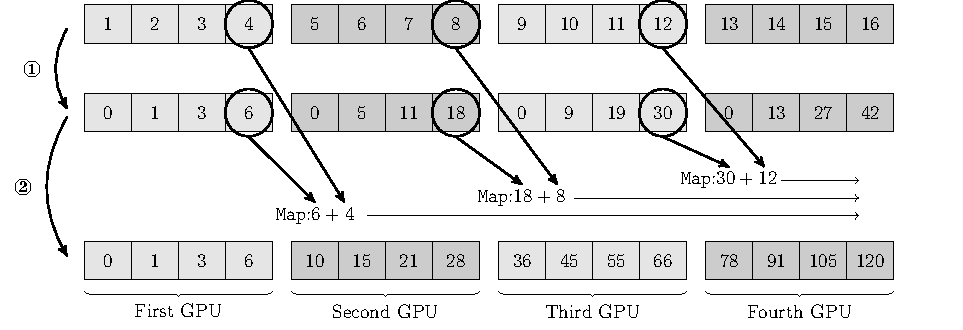
\includegraphics[width=.9\textwidth]{ASHES/scan}
    \caption{Scan on four GPUs: (1) All GPUs scan their parts independently.
            (2) map skeletons are created automatically and
             executed to produce the result.}
    \label{fig:scan}
\end{figure*}

\subsection{Skeletons for Multiple GPUs}
\label{sec:multi-gpu_skeletons}

The skeletons of SkelCL possess specific features for working in multi-GPU systems.
They take into account the distribution of their input vectors: each GPU that holds a part or a complete copy of a vector is involved in the execution of the skeleton.
Therefore, all GPUs automatically cooperate in the skeleton execution if its input vector is \emph{block}-distributed, whereas the skeleton is executed on one GPU if the vector distribution is \emph{single}.
If a skeleton's input vector is \emph{copy}-distributed, then all GPUs execute the same skeleton on their own copies.

Vectors can be passed to skeletons either as main inputs or as additional arguments.
For main input vectors, a skeleton-specific default distribution is set automatically by SkelCL, but the programmer can override the defaults, i.\,e., specify a distribution that fits best for the application.
For vectors passed as an additional argument, no meaningful default distribution can be provided by the system, because the access pattern for the vector is determined by the user-defined function.
Therefore, the user has to specify explicitly the distribution for these vectors.

\subsection{Implementation of Skeletons on Multiple GPUs}

\paragraph{Map and zip}
In a multi-GPU setting, each GPU executes the map's unary function on its part of the input vector.
The same holds for the zip skeleton, but it requires both input vectors to have the same distribution, and, in case of the single-distributed vectors, they also have to be stored on the same GPU.
If this requirement is not satisfied, SkelCL automatically changes the input vector distribution to block distribution.
This distribution is also set by default for input vectors with no distribution specified by the user.
Both, the map and zip skeleton, set their output vector distribution to that of their input vectors.

\paragraph{Reduce}
The reduce skeleton automatically performs all necessary synchronization and communication between CPU and GPUs, in three steps:
\begin{enumerate}
 \item Every GPU executes a local reduction for its local part of data;
 \item The results of all GPUs are gathered by the CPU;
 \item The CPU reduces these intermediate results to compute the final result.
\end{enumerate}
The output vector of the reduce skeleton holds only a single element, therefore, the output vector distribution is set to single.

\paragraph{Scan}
An example of the scan skeleton executed on four devices using addition as operation is shown in Figure~\ref{fig:scan}.
The input vector $[1,\ldots,16]$ is distributed using the \emph{block} distribution by default (shown in the top line).
After performing the scan algorithm on all devices (second line of the figure), map skeletons are built implicitly using the marked values and executed on all devices except the first one.
This produces the final result, as shown in the bottom line.

The SkelCL implementation of the scan skeleton assumes the GPUs to have a fixed order, such that each GPU (except the first one) has a predecessor:
\begin{enumerate}
 \item Every GPU executes a local scan algorithm for its local part of data;
 \item The results of all GPUs are downloaded to the host;
 \item For each GPU (except the first one), a map skeleton is implicitly created that combines the result of the GPU's predecessors with all elements of its part using the user-defined operation of the scan skeleton;
 \item The newly created map skeletons compute the final results on all GPUs.
\end{enumerate}
The output vector is block-distributed among all GPUs.
\from{ASHES end}




\from{Paraphrase begin}
\section{SkelCL (Paraphrase)}

\subsection{Algorithmic Skeletons}

% EXAMPLE
Listing~\ref{lst:dotproduct} shows how a dot product of two vectors is implemented in SkelCL using two skeletons:
the \emph{Zip} skeleton is customized by usual multiplication, and the \emph{Reduce} skeleton is customized by usual addition.
This program comprises 8 lines of code (omitting comments and empty lines).
\begin{lstlisting}[%
caption={SkelCL program computing the dot product of two vectors.},%
float=tbp,%
label={lst:dotproduct}]
int main (int argc, char const* argv[]) {
  SkelCL::init();                  /* initialize SkelCL */
  Reduce<float> sum (              /* create skeletons */
    "float func(float x,float y) { return x+y; }" );
  Zip<float> mult (
    "float func(float x, float y) { return x*y; }" );
                                   /* create input vectors */
  Vector<float> A(SIZE); fillVector(A);
  Vector<float> B(SIZE); fillVector(B);
                                   /* execute skeletons */
  Vector<float> C = sum( mult( A, B ) );
  cout << "Result: " << C.front(); /* print result */ }
\end{lstlisting}
For comparison, an OpenCL-based implementation of a dot product provided in the NVIDIA SDK~\cite{CUDASDK-10} requires 68 lines of code (kernel function: 9~lines, host program: 59~lines).
Besides, additional code would be necessary for a multi-device implementation, including statements for data transfer between multiple devices and for splitting input data and merging output data on the host.

In SkelCL, skeletons can be executed on single- and multi-device systems.
In case of a multi-device system, the calculation specified by a skeleton is performed automatically on all devices available to the system.
The SkelCL program in Listing~\ref{lst:dotproduct} can thus be executed on a multi-device system without any change.

\subsection{The MapOverlap Skeleton}
Many applications dealing with two-dimensional data perform calculations for every data element taking neighboring data elements into account.
For example, image processing algorithms, like the gaussian blur, calculate a new value for every pixel of an input image using the previous value of the pixel and its surrounding values.

To facilitate the development of such applications, we extend SkelCL by an additional skeleton in combination with a new matrix data type, which is presented in Section~\ref{sec:skelcl:matrix}.
This skeleton can be used with either vector or matrix data type.
We explain the details of the new skeleton for the matrix data type.
\begin{itemize}
  \item The \emph{MapOverlap} skeleton takes two parameters: a function $f$ and an integer value $d$.
   It applies $f$ to each element of an input matrix $m_{in}$ while taking the neighboring elements within the range $[-d, +d]$ in each dimension into account, i.\,e.
  \begin{align*}
m_{out}[i,j]=f\left(
\begin{array}{ccccc}
m_{in}[i-d,j-d] & \hdots & m_{in}[i-d,j] & \hdots & m_{in}[i-d,j+d] \\
\vdots & ~ & \vdots & ~ & \vdots \\
m_{in}[i,j-d] & \hdots & m_{in}[i,j] & \hdots & m_{in}[i,j+d]\\
\vdots & ~ & \vdots & ~ & \vdots \\
m_{in}[i+d,j-d] & \hdots & m_{in}[i+d,j] & \hdots & m_{in}[i+d,j+d] \\
\end{array}
\right)
\end{align*}
\end{itemize}

In the actual source code, the application developer provides the function $f$ which receives a pointer to the element in the middle, $m_{in}[i,j]$.
Listing~\ref{lst:mapoverlap01} shows a simple example of computing the sum of all direct neighboring values using the MapOverlap skeleton.
To access the elements of the input matrix $m_{in}$, function \texttt{get} is used, as provided by SkelCL.
All indices are specified relative to the middle element $m_{in}[i,j]$, therefore, for accessing this element the function call \texttt{get(m\_in, 0, 0)} is used.

The application developer must ensure that only elements in the range specified by the second argument $d$ of the MapOverlap skeleton, are accessed.
In Listing~\ref{lst:mapoverlap01}, range is specified as $d=1$, therefore, only direct neighboring elements are accessed.
To enforce this property, boundary checks are performed at runtime by the \texttt{get} function.
In future work, we plan to avoid boundary checks at runtime by statically proving that all memory accesses are in bounds, as it is the case in the shown example.

Special handling is necessary when accessing elements out of the boundaries of the matrix, e.g., when the item in the top-left corner of the matrix accesses elements above and left of it.
The MapOverlap skeleton can be configured to handle such out-of-bound memory accesses in two possible ways:
1) a specified neutral value is returned;
2) the nearest valid value inside the matrix is returned.
In Listing~\ref{lst:mapoverlap01}, the first option is chosen and $0.0$ is provided as neutral value.

\begin{lstlisting}[%
caption={MapOverlap skeleton computing the sum of all direct neightbors for every element in a matrix},%
float=tbp,%
label={lst:mapoverlap01}]
MapOverlap<float(float)> m("float func(float* m_in){
     float sum = 0.0f;
     for (int i = -1; i < 1; ++i)
       for (int j = -1; j < 1; ++i)
         sum += get(m_in, i, j);
     return sum;
   }", 1, SCL_NEUTRAL, 0.0f);
\end{lstlisting}

Listing~\ref{lst:raw_opencl01} shows how the same simple calculation can be performed in standard OpenCL.
While the amount of lines of code increases by a factor of 2, the complexity of each single line also increases, as follows.
Besides a pointer to the output memory, the width of the matrix has to be provided as parameter.
The correct index has to be calculated for every memory access using an offset and the width of the matrix.
Therefore, knowledge about how the two-dimensional matrix is stored in one-dimensional memory is required.
In addition, manual boundary checks have to be performed to avoid faulty memory accesses.\bigskip

\begin{lstlisting}[%
caption={An OpenCL kernel performing the same calculation as the MapOverlap skeleton shown in Listing~\ref{lst:mapoverlap01}.\bigskip},%
label={lst:raw_opencl01}]
__kernel void sum_up(__global float* m_in,
                     __global float* m_out,
                     int width, int height) {
  int i_off = get_global_id(0); int j_off = get_global_id(1);
  float sum = 0.0f;
  for (int i = i_off - 1; i < i_off + 1; ++i)
    for (int j = j_off - 1; j < j_off + 1; ++j) {
      // perform boundary checks
      if ( i < 0 || i > width || j < 0 || j > height )
        continue;
      sum += m_in[ j * width + i ];     }
  m_out[ j_off * width + i_off ] = sum; }
\end{lstlisting}

SkelCL avoids all these low-level details.
Neither additional parameter, nor index calculations or manual boundary checks are necessary.
In SkelCL, the application developer only provides the source code implementing the steps required by the algorithm.

\subsection{Data distribution on multiple devices}
\label{sec:data_distribution}
The key feature of SkelCL for multi-device systems is that SkelCL's data types abstract from memory ranges on multiple devices, i.\,e. the data is accessible by each device.
However, each device may access different parts of a container (vector or matrix) or may even not access it at all.
For example, when implementing work-sharing on multiple devices, the devices will usually access disjoint parts of input data, such that copying only a part of the container to a device would be more efficient than copying the whole data to each device.

To simplify the specification of partitionings of containers in programs for multi-device systems, SkelCL implements the \emph{distribution} mechanism that describes how a container is distributed among the available devices.
It allows the programmer to abstract from managing memory ranges which are shared or spread across multiple devices:
the programmer can think of a distributed container as of a self-contained entity.

Four kinds of distribution are currently implemented in SkelCL and offered to the programmer:
\emph{block}, \emph{copy}, \emph{single} and \emph{overlap} (see Figure~\ref{fig:distributions}).
With \emph{block} distribution (Figure~\ref{fig:distributions:block}), each device stores a contiguous, disjoint part of the container.
The \emph{copy} distribution (Figure~\ref{fig:distributions:copy}) copies container's entire data to each available device.
In case of \emph{single} distribution (Figure~\ref{fig:distributions:single}), container's whole data is stored on a single device (the first device by default).

Together with the matrix data type, we introduce a new distribution called \emph{overlap} (Figure~\ref{fig:distribution:overlap}).
The overlap distribution splits the matrix into one chunk for each device, similarly to the block distribution.
In addition to the block distribution, the following holds for an overlap-distributed matrix:
each chunk consists of a number of continuous rows, and, a parameter -- the \emph{overlap size} -- specifies the number of rows at the edges of a chunk which are copied to the two neighboring devices.
Figure~\ref{fig:distribution:overlap} illustrates the overlap distribution:
Device 0 receives the top chunk ranging from the top row to the middle, while device 1 receives the second chunk ranging from the middle row to the bottom.
The marked regions are the \emph{overlap regions} which are available on both devices.

The \emph{overlap} distribution is automatically selected as distribution by the MapOverlap skeleton, to ensure that every device has access to the neighboring elements as needed by the MapOverlap skeleton.

A programmer can set the distribution of containers explicitly, or every skeleton selects a default distribution for its input and output containers otherwise.
Container's distribution can be changed at runtime.
A change of distribution implies data exchanges between multiple devices and the host, which are performed by SkelCL implicitly and lazily, as described above.
Implementing such data transfers in the standard OpenCL is a cumbersome task:
data has to be downloaded to the host before it can be uploaded to other devices, including the corresponding length and offset calculations;
this results in a lot of low-level code which is completely hidden when using SkelCL.
\from{Paraphrase end}




\from{ICCS begin}
\section{The SkelCL Programming Model and the SkelCL Library (ICCS)}


\subsection{Data Distributions}
\label{sec:data_distribution}
For multi-GPU systems, SkelCL's parallel container data types (vector and matrix) abstract from the separate memory areas on multiple GPUs, i.\,e., container's data is accessible by each GPU.
To simplify the partitioning of a container on multiple GPUs, SkelCL supports the concept of \emph{distribution} that specifies how a container is distributed among the GPUs.
It allows the application developer to abstract from managing memory ranges which are shared or partitioned across multiple GPUs.

\begin{figure}[tb]
  \centering
  \begin{subfigure}{.22\textwidth}
    \includegraphics[width=\textwidth]{ICCS/singleDistribution}
    \caption{\emph{single}}
    \label{fig:distributions:single}
  \end{subfigure}
  \hfill
  \begin{subfigure}{.22\textwidth}
    \includegraphics[width=\textwidth]{ICCS/copyDistribution}
    \caption{\emph{copy}}
    \label{fig:distributions:copy}
  \end{subfigure}
  \hfill
  \begin{subfigure}{.22\textwidth}
    \includegraphics[width=\textwidth]{ICCS/blockDistribution}
    \caption{\emph{block}}
    \label{fig:distributions:block}
  \end{subfigure}
  \hfill
  \begin{subfigure}{.22\textwidth}
    \includegraphics[width=\textwidth]{ICCS/overlapDistribution}
    \caption{\emph{overlap}}
    \label{fig:distributions:overlap}
  \end{subfigure}
  \caption{Distributions of a vector in SkelCL.}
  \label{fig:distributions}
\end{figure}

Four kinds of distribution are currently available to the application developer in SkelCL:
\emph{single}, \emph{copy}, \emph{block}, and \emph{overlap} (see Fig.~\ref{fig:distributions} for illustration on a system with two GPUs).
If set to the \emph{single} distribution (Fig.~\ref{fig:distributions:single}), container's whole data is stored on a single GPU (the first GPU if not specified otherwise).
The \emph{copy} distribution (Fig.~\ref{fig:distributions:copy}) copies container's entire data to each available GPU.
With the \emph{block} distribution (Fig.~\ref{fig:distributions:block}), each GPU stores a contiguous, disjoint block of the container.
The \emph{overlap} distribution (Fig.~\ref{fig:distributions:overlap}) is used for the mapOverlap skeleton:
it stores on both GPUs a common block of data from the border between the GPUs.
The application developer can set the distribution of containers explicitly or every skeleton selects a default distribution for its input and output containers otherwise.
The distribution of a container can be changed at runtime:
this implies data exchanges between multiple GPUs and the CPU, which are performed by the SkelCL implementation implicitly.
As shown in Listing~\ref{lst:redistribution}, implementing such data transfers in the standard OpenCL is a cumbersome task:
data has to be downloaded to the CPU before it can be uploaded to other GPUs, including the corresponding length and offset calculations;
this results in a lot of low-level code which is completely hidden when using SkelCL.

\from{ICCS end}




\from{HLPP begin}
\section{The Allpairs Skeleton and its Implementation (HLPP)}
\label{sec:allpairs_skeleton}

\label{sec:formal_def}
We define the allpairs computation pattern for two sets of entities, each entity represented by a vector of length $d$.
Let the cardinality of the first set be $n$ and the cardinality of the second set be $m$.
We model the first set as a $n\times d$ matrix $A$ and the second set as a $m\times d$ matrix $B$.
The allpairs computation yields an output matrix $C$ of size $n\times m$ as follows:
$c_{i, j} = A_i \oplus B_j$, where $A_i$ and $B_j$ are row vectors of $A$ and $B$, correspondingly:
$A_i = [A_{i,1}, \cdots, A_{i, d}]$, $B_j = [B_{j,1}, \cdots, B_{j,d}]$, and $\oplus$ is a binary operator defined as vectors.

\begin{definition}
  \label{def:allpairs}
  Let $A$ be a $n\times d$ matrix, $B$ be a $m\times d$ matrix, and $C$ be a $n\times m$ matrix, with their elements $a_{i,j}$, $b_{i,j}$, and $c_{i,j}$ respectively.
  The algorithmic skeleton \emph{allpairs} with customizing binary function $\oplus$ is defined as follows:
  \[
    \allpairs(\oplus)\left(
      \left[ \begin{array}{ccc}%
 	      a_{1,1} & \cdots & a_{1,d}\\[.25em]
       	\vdots & & \vdots\\[.25em]
       	a_{n,1} & \cdots & a_{n,d}%
     	\end{array}\right],%
      \left[ \begin{array}{ccc}%
       	b_{1,1} & \cdots & b_{1,d}\\[-.25em]
       	\cdot & & \cdot\\[-.75em]
       	\cdot & & \cdot\\[-.25em]
       	b_{m,1} & \cdots & b_{m,d}%
   	\end{array}\right]\right)%
  	\eqdef 
      \left[ \begin{array}{ccc}%
 	      c_{1,1} & \cdots & c_{1,m}\\[.25em]
       	\vdots & & \vdots\\[.25em]
        c_{n,1} & \cdots & c_{n,m}%
   	\end{array}\right]
  \]
  where elements $c_{i,j}$ of the $n\times m$ matrix $C$ are calculated as follows:
  \[
	  c_{i,j} = \DottedVector{a_{i,1}}{a_{i,d}} \oplus \DottedVector{b_{j,1}}{b_{j,d}}
  \]
\end{definition}

Figure~\ref{fig:allpairs_access_a} illustrates this definition:
the element $c_{2,3}$ of matrix $C$ marked as \circled{3} is computed by combining the second row of $A$ marked as \circled{1} with the third row of $B$ marked as \circled{2} using the binary operator $\oplus$.
Figure~\ref{fig:allpairs_access_b} shows the same computation with the transposed matrix $B$.
\begin{figure}[b]
  \centering
	\includegraphics[width=0.44\textwidth]{HLPP/allpairs_access_pattern_alternative}
	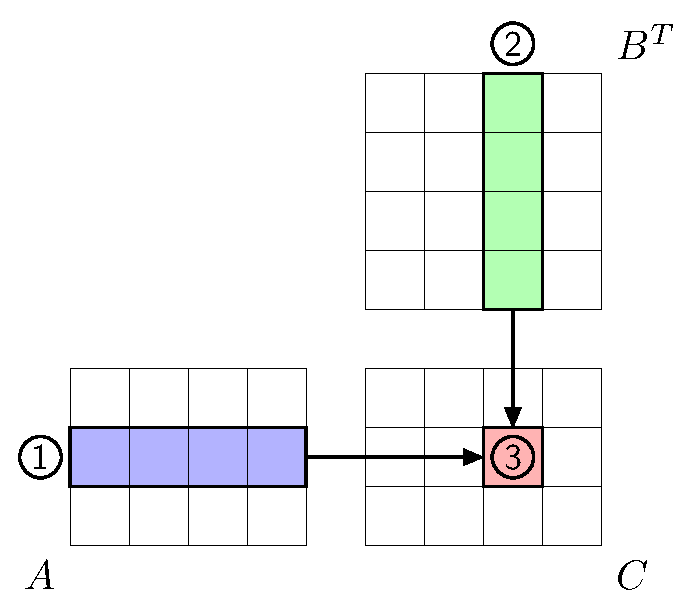
\includegraphics[width=0.44\textwidth]{HLPP/allpairs_access_pattern}
  \caption{The allpairs computation. Left: element $c_{2,3}$
    (\protect\tikz[baseline=(char.base)]\protect\node[shape=circle,draw,inner sep=1pt] (char) {3};)
    is computed by combining the second row of $A$
    (\protect\tikz[baseline=(char.base)]\protect\node[shape=circle,draw,inner sep=1pt] (char) {1};)
    with the third row of $B$
    (\protect\tikz[baseline=(char.base)]\protect\node[shape=circle,draw,inner sep=1pt] (char) {2};)
    using the binary operator $\oplus$. Right: the transposed matrix $B$ is used.}
  \label{fig:allpairs_access}
\end{figure}

\vspace{6em}
Let us consider two example applications which can be expressed by customizing the allpairs skeleton with a particular function $\oplus$.

\paragraph{Example 1:}
The Manhattan distance (or $L_1$ distance) is a measure of distance which is used in many applications.
In general, it is defined for two vectors, $v$ and $w$, of equal length $d$, as follows:
\begin{equation}
  \label{eq:man_dist}
  \ManDist(v, w) = \sum_{k=1}^d | v_k - w_k | 
\end{equation}
In~\cite{DaDQR-09}, the so-called Pairwise Manhattan Distance (\emph{PMD}) is studied as a fundamental operation in hierarchical clustering for data analysis.
\emph{PMD} is obtained by computing the Manhattan distance for every pair of rows of a given matrix.
This computation for arbitrary matrix $A$ can be expressed using the allpairs skeleton customized with the Manhattan distance defined in (\ref{eq:man_dist}):
\begin{equation}
  \PMD(A) = \mbox{\emph{allpairs}}(\mbox{\emph{ManDist}})\left(A, A\right)
\end{equation}
The $n\times n$ matrix computed by the customized skeleton contains the Manhattan distance for every pair of rows of the input $n\times d$ matrix $A$.

\paragraph{Example 2:}
Matrix multiplication is a basic linear algebra operation, which is a building block of many scientific applications.
An $n\times d$ matrix $A$ is multiplied by a $d\times m$ matrix $B$, producing a $n\times m$ matrix $C=A\times B$ whose element $c_{i,j}$ is computed as the dot product of the $i$th row of $A$ with the $j$th column of $B$.
The dot product of two vectors $a$ and $b$ of length $d$ is computed as:
\begin{equation}
  \dotProduct (a,b) = \sum_{k=1}^d a_k \cdot b_k
\end{equation}
The matrix multiplication can be expressed using the allpairs skeleton as:
\begin{equation}
  A\times B = \allpairs(\dotProduct)\left(A, B^T\right)
  \label{eq:mat_mult_allpairs}
\end{equation}
where $B^T$ is the transpose of matrix $B$.
We will use the matrix multiplication as our running example for the allpairs skeleton throughout the paper.

\vspace{1em}
We develop the allpairs skeleton within the skeleton library SkelCL~\cite{StKG-12}, which is built on top of OpenCL and targets modern parallel systems with multiple GPUs.
Currently, five other skeletons are available in SkelCL: \emph{map}, \emph{zip}, \emph{reduce}, \emph{scan}, and \emph{mapOverlap}.
Skeletons operate on container data types (in particular vectors and matrices) which alleviate the memory management of GPUs:
data is copied automatically to and from GPUs, instead of manually performing data transfers as required in OpenCL.
For programming multi-GPU systems, SkelCL offers the application programmer a data distribution mechanism to specify how the data of a container is distributed among the GPUs in the system.
The container's data can either be assigned to a single GPU, be copied to all GPUs, or be partitioned in equal blocks across the GPUs, possibly with an overlap.
If the data distribution is changed in the program, the necessary data movements are done automatically by the system~\cite{StKG-12}.

\begin{lstlisting}[%                                                             
caption={Matrix multiplication in SkelCL using the \emph{allpairs} skeleton.},%
float=t,%                                                                       
numbers=left,%
label={lst:basic_mm}]
skelcl::init();
Allpairs<float(float, float)> mm(
 "float func(float_matrix_t a, float_matrix_t b) {\
  float c = 0.0f;\
  for (int i = 0; i < width(a); ++i) {\
    c += getElementFromRow(a, i) * getElementFromCol(b, i); }\
  return c; }");
Matrix<float> A(n, k); fill(A);
Matrix<float> B(k, m); fill(B);
Matrix<float> C = mm(A, B);
\end{lstlisting}

Listing~\ref{lst:basic_mm} shows the SkelCL program for computing matrix multiplication using the \emph{allpairs} skeleton;
the code follows directly from the mathematical formulation (\ref{eq:mat_mult_allpairs}).
In the first line, the SkelCL library is initialized.
Skeletons are implemented as classes in SkelCL and customized by instantiating a new object, like in line 2.
The \texttt{Allpairs} class is implemented as a template class specified with the data types of matrices involved in the computation (\texttt{float(float, float)}).
This way the implementation can ensure the type correctness by checking the types of the arguments when the skeleton is executed in line 10.
The customizing function -- specified as a string (line 3 -- 7) -- is passed to the constructor.
Data types for matrices (\texttt{float\_matrix\_t} in line 3) are defined by the SkelCL implementation and used as arguments of helper functions for accessing elements from both matrices (line 6).
The transpose of matrix $B$ required by the definition (\ref{eq:mat_mult_allpairs}) is implicitly performed by accessing elements from the columns of $B$ using the helper function \texttt{getElementFromCol}.
After initializing the two input matrices (line 8 and 9), the calculation is performed in line 10.

In our SkelCL library, skeletons are implemented by translating them into executable OpenCL code.
Listing~\ref{lst:basic_impl} shows the OpenCL kernel which is combined with the given customizing function by the implementation of the allpairs skeleton.
The customizing function (named \texttt{\emph{func}} in Listing~\ref{lst:basic_mm}) is renamed to match the name used in the function call in the implementation (\texttt{USER\_FUNC} in Listing~\ref{lst:basic_impl}).
In addition, the types used in the predefined OpenCL kernel (\texttt{TYPE\_LEFT}, \texttt{TYPE\_RIGHT}, and \texttt{TYPE\_OUT} in Listing~\ref{lst:basic_impl}) are adjusted to match the actual types of the elements used in the computation (in this case, all three types are \texttt{float}).
These modifications ensure that a valid OpenCL program performing the allpairs calculation is constructed.
This generated OpenCL program is executed once for every element of the output matrix $C$.
In lines 6 -- 7, the implementation prepares variables (\texttt{Am} and \texttt{Bm}) of a predefined data type (\texttt{float\_matrix\_t}) which encapsulate the matrices $A$ and $B$ and passes them to the customizing function which is called in line 9.

\begin{lstlisting}[%                                                             
caption={Generic OpenCL kernel used in the implementation of the allpairs skeleton.},%
float=t,%                                                                       
numbers=left,%
label={lst:basic_impl}]
__kernel void allpairs(const __global TYPE_LEFT*  A,
                       const __global TYPE_RIGHT* B,
                             __global TYPE_OUT*   C,
                             int n, int d, int m) {
  int col = get_global_id(0); int row = get_global_id(1);
  float_matrix_t Am; Am.data = A; Am.width = d; Am.row = row;
  float_matrix_t Bm; Bm.data = B; Bm.width = m; Bm.col = col;
  if (row < n && col < m)
    C[row * m + col] = USER_FUNC(Am, Bm); }
\end{lstlisting}

To achieve high performance, skeleton implementations must efficiently exploit the complex memory hierarchy of multi-GPU architectures.
There are two main types of memory in OpenCL: \emph{global} and \emph{local memory}.
The global memory is typically large but slow; the local memory is small but fast and has similar performance as caches in traditional systems, but has to be programmed manually.
On modern GPUs, accesses to the global memory are very expensive, taking up to 800 processor cycles, as compared to only few cycles required to access the local memory~\cite{NVIDIA-12}.

The generic implementation of the allpairs skeleton in Listing~\ref{lst:basic_impl} makes no assumption about the order in which the customizing function (\texttt{USER\_FUNC}) accesses the elements of its two input vectors.
In this general case, we cannot assume that the two vectors fit entirely into the restricted GPU local memory.
Therefore, we have to use only the global memory in the generic implementation.
To improve our implementation of the allpairs skeleton, we restrict the memory access pattern of the customizing function in the next section.


\section{The Specialized Allpairs Skeleton (HLPP)}
\label{sec:opt_allpairs_skeleton}
In this section, we first analyze the memory access pattern of the matrix multiplication and then observe that this pattern can also be found in some other allpairs computations.
We, therefore, define a specialized version of the allpairs skeleton, which is suitable for applications having this pattern, and show how it can be implemented more efficiently than the generic skeleton.

\subsection{The memory access pattern of the matrix multiplication}
Figure~\ref{fig:single_memory_access} shows the memory access pattern of the matrix multiplication for $4\times 4$ matrices.
\begin{figure}[t]
  \centering
  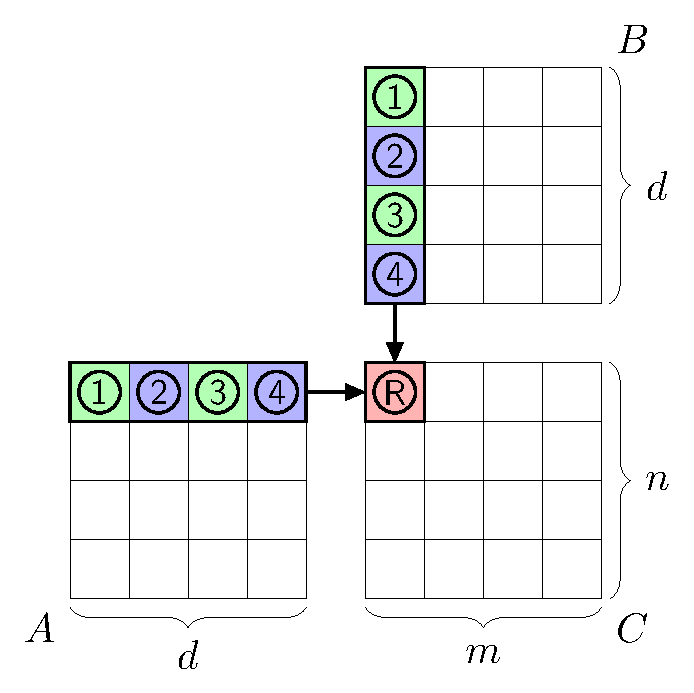
\includegraphics[width=0.4\textwidth]{HLPP/single_memory_access}
  \caption{Memory access pattern of the matrix multiplication $A\times B = C$.}
  \label{fig:single_memory_access}
\end{figure}
To compute the element \circled{R} of the result matrix $C$, the first row of matrix $A$ and the first column of matrix $B$ are needed.
In the skeleton-based code, these two vectors are used by the customizing function (which is the dot product) for pairwise computations:
the two elements marked as \circled{1} are multiplied and the intermediate result is stored;
then, the next elements (marked as \circled{2}) are multiplied and the result is added to the intermediate result, and so forth.
Let us estimate the number of global memory accesses for computing an element of the matrix multiplication in the generic implementation (Listing~\ref{lst:basic_impl}).
One global memory read access for every element of both input vectors is performed, and a single global memory write access is required to write the result into the output matrix.
Therefore, $n\cdot m\cdot (d + d + 1)$ global memory accesses are performed in total, where $n$ and $m$ are the height and width of matrix $C$ and $d$ is the width of $A$ and the height of $B$.

Obviously, the customizing function of the pairwise Manhattan distance (Example 1 in Section~\ref{sec:allpairs_skeleton}) follows the same memory access pattern as matrix multiplication.
To find a common representation for a customizing function with this pairwise access pattern, we describe it as a combination of two well-known algorithmic skeletons: \emph{zip} and \emph{reduce}.

The \emph{zip} skeleton combines two input vectors by applying its customizing function ($\odot$) pairwise, producing the result vector:
\[ \zip\ (\odot)\ \DottedVector{a_1}{a_n}\ \DottedVector{b_1}{b_n}\ =\ \DottedVector{a_1 \odot b_1}{a_n \odot b_n} \]

The \emph{reduce} skeleton transforms an input vector into a scalar value by repeatedly applying its binary associative customizing operator ($\oplus$):
\[ \reduce\ (\oplus)\ \DottedVector{a_1}{a_n}\ =\ a_1 \oplus a_2 \oplus \cdots \oplus a_n \]

It is possible to sequentially compose these two customized skeletons.
For two functions $f: X \to Y$ and $g: Y\to Z$, the \emph{sequential composition} denoted by $g \circ f: X \to Z$ means that $f$ is applied first and then $g$ is applied to the return value of $f$ as input: $(g\circ f)(x) = g(f(x))$.
Our customized skeletons are functions with types that allow their composition as follows:
\begin{eqnarray*}
  (reduce\ (\oplus) \circ zip\ (\odot) ) \DottedVector{a_1}{a_n}\ \DottedVector{b_1}{b_n} &=& \\
  reduce\ (\oplus) \left( zip\ (\odot) \DottedVector{a_1}{a_n}\ \DottedVector{b_1}{b_n} \right) &=& (a_1 \odot b_1) \oplus \cdots \oplus (a_n \odot b_n)
\end{eqnarray*}
This composition of the two customized skeletons yields a function which takes two input vectors and produces a single scalar value:
\begin{equation}
  zipReduce\ (\oplus, \odot)\ a\ b = 
  \left( reduce\ (\oplus) \circ zip\ (\odot) \right)\ a\ b
\end{equation}

Following the definition of {\zipReduce}, we can express the customizing function of the Manhattan distance as follows.
We use the binary operator $a \ominus b = |a - b|$ as customizing function for zip, and addition as customizing function for the reduce skeleton:
\begin{eqnarray*}
    ManDist(a, b) = \sum_{i=1}^{n} | a_i - b_i | &=&
    (a_1 \ominus b_1) + \cdots + (a_n \ominus b_n) \\
    &=& zipReduce(+, \ominus)\ \DottedVector{a_1}{a_n}\ \DottedVector{b_1}{b_n}
\end{eqnarray*}

Similarly, we can express the dot product (which is the customizing function of matrix multiplication) as a zip-reduce composition, by using multiplication for customizing zip and addition for customizing the reduce skeleton:
\begin{eqnarray*}
  \dotProduct(a, b) = \sum_{i = 1}^{n} a_i \cdot b_i &=& (a_1 \cdot b_1) + \cdots + (a_n \cdot b_n) \\
  &=& zipReduce(+, \cdot)\ \DottedVector{a_1}{a_n}\ \DottedVector{b_1}{b_n}
\end{eqnarray*}

We can now specialize the generic Definition~\ref{def:allpairs} by employing the sequential composition of the customized reduce and zip skeletons for customizing the allpairs skeleton.
From here on, we refer to this specialization as the allpairs skeleton \emph{customized with zip-reduce}.

While not every allpairs computation can be expressed using the specialization, many real-world problems can.
In addition to the matrix multiplication and the pairwise Manhattan distance examples are the pairwise computation of the Pearson correlation coefficient~\cite{DaDQR-09} and estimation of Mutual Informations~\cite{DaSSK-04}.
The composition of zip and reduce is well known in the functional programming world.
Google's popular MapReduce programming model has been inspired by a similar composition of the \emph{map} and reduce skeletons; see~\cite{La-07}~for the relation of MapReduce to functional programming.

\begin{lstlisting}[%                                                             
caption={Matrix multiplication in SkelCL using the specialized \emph{allpairs} skeleton.},%
float=b,%                                                                       
numbers=left,%
label={lst:nested_allpairs}]
skelcl::init();
Zip<float(float, float)> mult
    ("float func(float x, float y) { return x*y; }");
Reduce<float(float, float)> sum_up
    ("float func(float x, float y) { return x+y; }");
Allpairs<float(float, float)> mm(sum_up, mult);
Matrix<float> A(n, d); fill(A);
Matrix<float> B(d, m); fill(B);
Matrix<float> C = mm(A, B);
\end{lstlisting}

Listing~\ref{lst:nested_allpairs} shows how the matrix multiplication can be programmed in SkelCL using the allpairs skeleton customized with zip-reduce.
In line 1, the SkelCL library is initialized.
In lines 2 and 3, the zip skeleton is defined using multiplication as customizing function and in lines 4 and 5, the reduce skeleton is customized with addition.
These two customized skeletons are passed to the allpairs skeleton on its creation in line 6.
The implementation of the allpairs skeleton then uses the two customizing functions of zip and reduce to generate the OpenCL kernel performing the allpairs computation.
In line 9, the skeleton is executed taking two input matrices and producing the output matrix.
Note that we create objects of the same \texttt{Allpairs} class when using the generic allpairs implementation (Listing~\ref{lst:basic_impl} line 2) and the specialized implementation (Listing~\ref{lst:nested_allpairs} line 6).
Depending on which of the overloaded constructors is used, either the generic or the specialized implementation is created.

\subsection{Implementation of the specialized allpairs skeleton}
By expressing the customizing function of the allpairs skeleton as a zip-reduce composition, we provide additional semantic information about the memory access pattern of the customizing function to the skeleton implementation, thus allowing for improving the performance.
Our idea of optimization is based on the OpenCL programming model that organizes \emph{work-items} (i.\,e., threads executing a kernel) in \emph{work-groups} which share the same GPU local memory.
By loading data needed by multiple work-items of the same work-group into the local memory, we can avoid repetitive accesses to the global memory.

\begin{figure}[b]
  \centering
  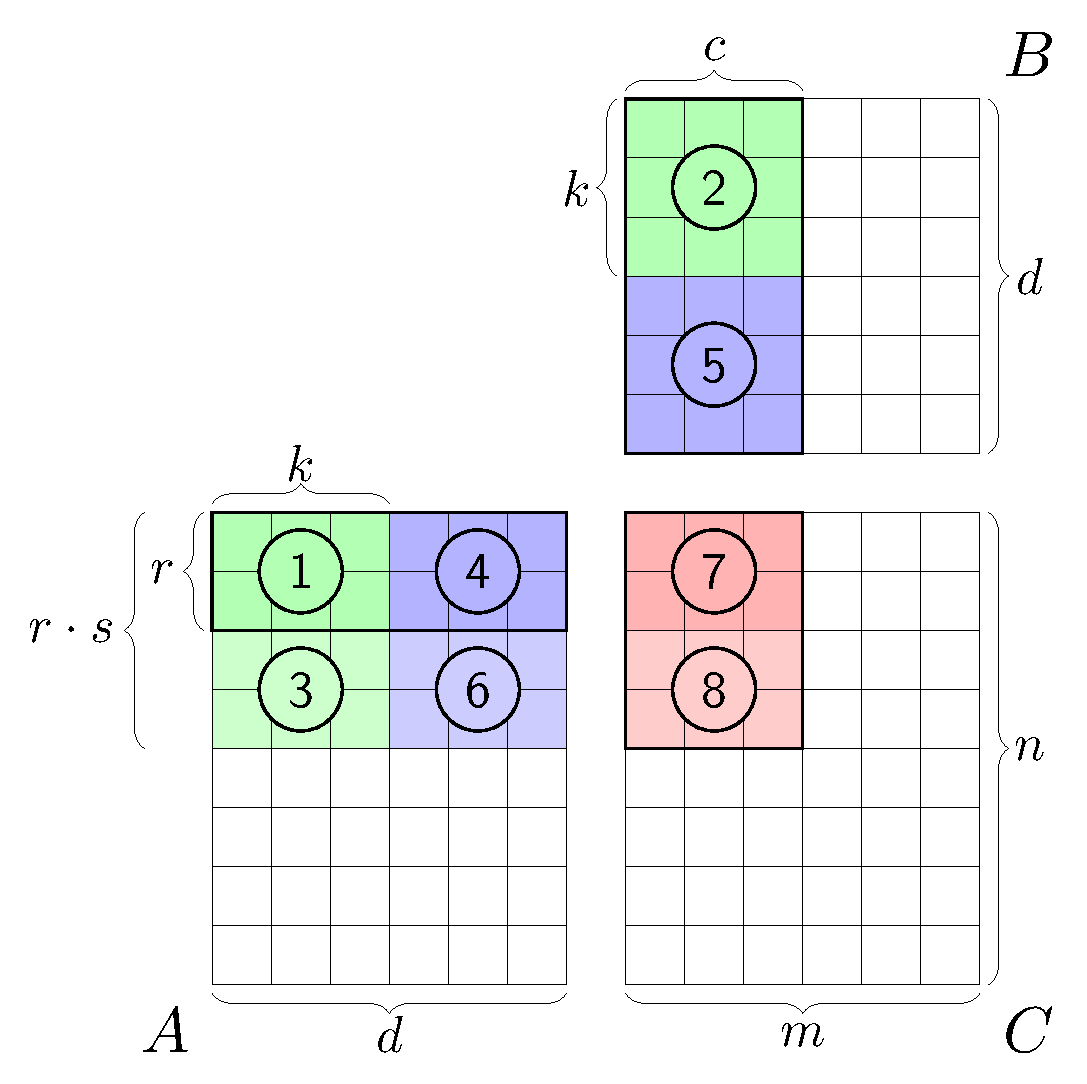
\includegraphics[width=.4\textwidth]{HLPP/memory_access}
  \caption{Implementation schema of the specialized allpairs skeleton.}
  \label{fig:memory_access}
\end{figure}
For the allpairs skeleton with the zip-reduce customizing function, we can adopt the implementation schema for GPUs~\cite{SaA-13}, as shown in Figure~\ref{fig:memory_access}.
We allocate two arrays in the local memory, one of size $r\times k$ ($r=2$, $k=3$ in Figure~\ref{fig:memory_access}) for elements of $A$ and one of size $k\times c$ ($c=3$ in Figure~\ref{fig:memory_access}) for elements of $B$.
A work-group consisting of $c\times r$ work-items computes $s$ blocks ($s=2$ in Figure~\ref{fig:memory_access}) of the result matrix $C$.
In Figure~\ref{fig:memory_access}, the two blocks marked as \circled{7} and \circled{8} are computed by the same work-group as follows.
In the first iteration, the elements of blocks \circled{1} and \circled{2} are loaded into the local memory and combined following the zip-reduce pattern.
The obtained intermediate result is stored in block \circled{7}.
Then, the elements of block \circled{3} are loaded and combined with the elements from \circled{2} which still reside in the local memory.
The intermediate result is stored in block \circled{8}.
In the second iteration, the algorithm continues in the same manner with blocks \circled{4}, \circled{5}, and \circled{6}, but this time, the elements of the blocks are also combined with the intermediate results of the first iteration, which are stored in blocks \circled{7} and \circled{8}.
The advantage of computing multiple blocks by the same work-group is that we keep the elements of $B$ in the local memory when computing the intermediate results, i.\,e., we do not reload block \circled{2} twice for the computation of blocks \circled{7} and \circled{8}.

Every element loaded from the global memory is used by multiple work-items:
e.\,g., the upper left element of block \circled{1} is loaded only once from the global memory, but used three times:
in the computation of the upper left, upper middle, and upper right elements of \circled{7}.
In general, every element loaded from $A$ is reused $c$ times, and every element from $B$ is reused $r\cdot s$ times.
As the intermediate results are stored in the global memory of matrix $C$, we perform two additional memory accesses (read/write) for every iteration, i.\,e., $2\cdot \frac{d}{k}$ in total.
Therefore, instead of $n\cdot m\cdot (d + d + 1)$ global memory accesses necessary when not using the local memory, only $n\cdot m\cdot (\frac{d}{r\cdot s} + \frac{d}{c} + 2\cdot \frac{d}{k})$ global memory accesses are performed.
By increasing the parameters $s$ and $k$, or the number of work-items in a work-group ($c$ and $r$), more global memory accesses can be saved.
However, the work-group size is limited by the GPU hardware.
While the parameters can be chosen independently of the matrix sizes, we have to consider the amount of available local memory.
\cite{SaA-13}~discusses how suitable parameters can be found by performing runtime experiments.

\begin{figure}[b]
  \centering
  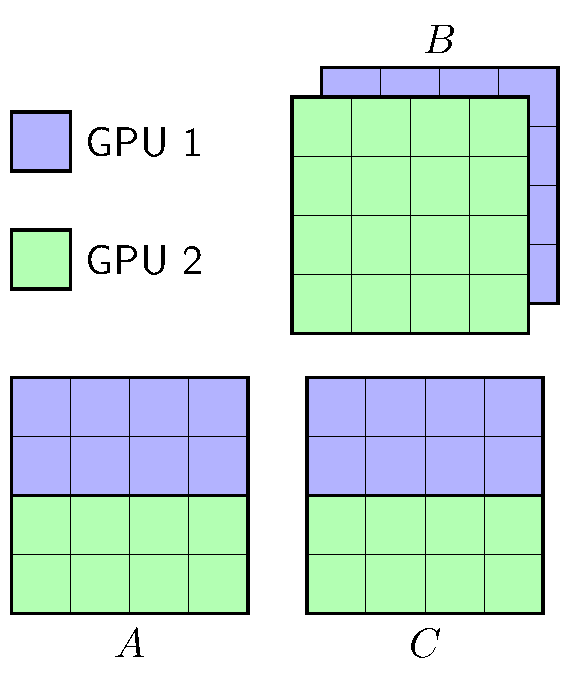
\includegraphics[width=.3\textwidth]{HLPP/multi_gpu}
  \caption{Data distributions used for a system with two GPUs: matrices $A$ and $C$ are block distributed, matrix $B$ is copy distributed.}
  \label{fig:multi_gpu}
\end{figure}

\section{The Allpairs Skeleton using Multiple GPUs (HLPP)}
\label{sec:multi_gpu}
The allpairs skeleton can be efficiently implemented not only on systems with a single GPU, but on multi-GPU systems as well.
The SkelCL library provides four \emph{data distributions} which specify how a container data type (vector or matrix) is distributed among multiple GPUs~\cite{StKG-12}.
We use two of them in our multi-GPU implementation of the allpairs skeleton, as shown in Figure~\ref{fig:multi_gpu}:
Matrix $B$ is \emph{copy} distributed, i.\,e., it is copied entirely to all GPUs in the system.
Matrix $A$ and $C$ are \emph{block} distributed, i.\,e., they are row-divided into as many equally-sized blocks as GPUs are available;
each block is copied to its corresponding GPU.
Following these distributions, each GPU computes one block of the result matrix $C$.
In the example with two GPUs shown in Figure~\ref{fig:multi_gpu}, the first two rows of $C$ are computed by GPU 1 and the last two rows by GPU 2.
The allpairs skeleton automatically selects these distributions; therefore, no changes to the already discussed implementations of the matrix multiplication are necessary for using multiple GPUs.
\from{HLPP end}


\from{PaCT begin}


\subsection{Data Distribution on Multiple GPUs}
In applications working on container data types (vectors, matrices, etc.) GPU's often access disjoint parts of input data, such that copying only a part of the container to a GPU would be more efficient than copying the whole data to each GPU. To simplify the specification of partitionings of containers in programs for multi-GPU systems, SkelCL implements the \emph{distribution} mechanism that describes how a container is distributed among the available GPUs.
It allows the programmer to abstract from managing memory ranges which are shared or spread across multiple GPUs:
the programmer can think of a distributed container as of a self-contained entity.

\begin{figure}[tb]
  \centering
  \begin{subfigure}{.22\textwidth}
    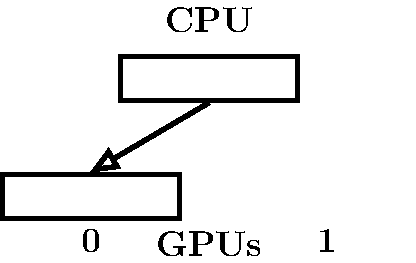
\includegraphics[width=\textwidth]{PaCT/singleDistribution_vector}
    \caption{\emph{single}}
    \label{fig:distributions:single}
  \end{subfigure}
  \hfill
  \begin{subfigure}{.22\textwidth}
    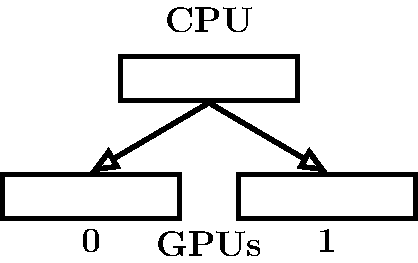
\includegraphics[width=\textwidth]{PaCT/copyDistribution_vector}
    \caption{\emph{copy}}
    \label{fig:distributions:copy}
  \end{subfigure}
  \hfill
  \begin{subfigure}{.22\textwidth}
    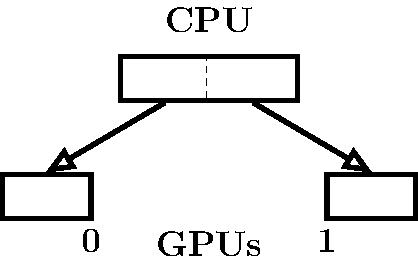
\includegraphics[width=\textwidth]{PaCT/blockDistribution_vector}
    \caption{\emph{block}}
    \label{fig:distributions:block}
  \end{subfigure}
  \hfill
  \begin{subfigure}{.22\textwidth}
    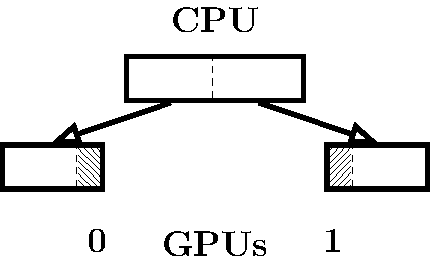
\includegraphics[width=\textwidth]{PaCT/overlapDistribution_vector}
    \caption{\emph{overlap}}
    \label{fig:distributions:overlap}
  \end{subfigure}
  \caption{Distributions of a vector in SkelCL.}
  \label{fig:distributions}
  \bigskip
\end{figure}

\begin{figure}[tbp]
  \centering
  \begin{subfigure}{.22\textwidth}
    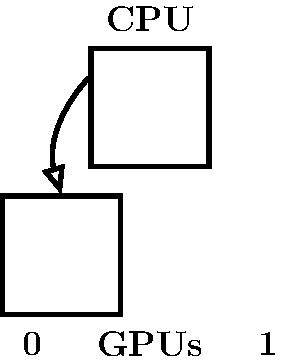
\includegraphics[width=\textwidth]{PaCT/singleDistribution_matrix}
    \caption{\emph{single}}
    \label{fig:Distribution_matrixs:single}
  \end{subfigure}
  \hfill
  \begin{subfigure}{.22\textwidth}
    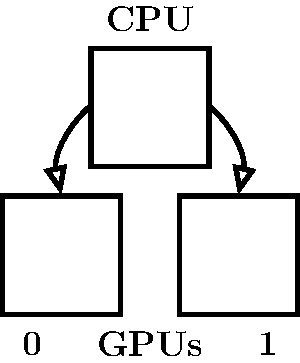
\includegraphics[width=\textwidth]{PaCT/copyDistribution_matrix}
    \caption{\emph{copy}}
    \label{fig:Distribution_matrixs:copy}
  \end{subfigure}
  \hfill
  \begin{subfigure}{.22\textwidth}
    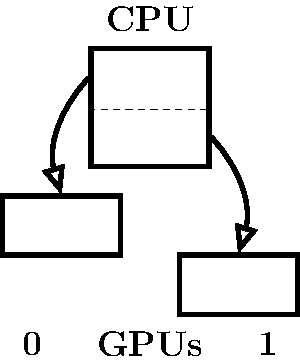
\includegraphics[width=\textwidth]{PaCT/blockDistribution_matrix}
    \caption{\emph{block}}
    \label{fig:Distribution_matrixs:block}
  \end{subfigure}
  \hfill
  \begin{subfigure}{.22\textwidth}
    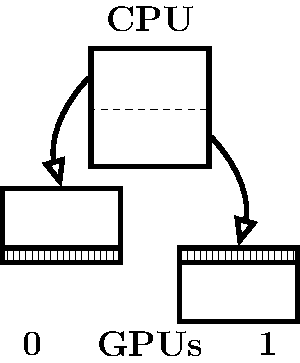
\includegraphics[width=\textwidth]{PaCT/overlapDistribution_matrix}
    \caption{\emph{overlap}}
    \label{fig:Distribution_matrixs:overlap}
  \end{subfigure}
  \caption{Distributions of a matrix in SkelCL.}
  \label{fig:distributions_matrix}
\end{figure}


Four kinds of distribution are currently available in SkelCL:
\emph{single}, \emph{copy}, \emph{block}, and \emph{overlap} (see Fig.~\ref{fig:distributions} for distributing a vector on a system with two GPUs).
If distribution is set to \emph{single} (Fig.~\ref{fig:distributions:single}), than vector's whole data is stored on a single GPU (the first GPU if not specified otherwise).
The \emph{copy} distribution (Fig.~\ref{fig:distributions:copy}) copies vector's entire data to each available GPU.
With the \emph{block} distribution (Fig.~\ref{fig:distributions:block}), each GPU stores a contiguous, disjoint chunk of the vector.
The \emph{overlap} distribution (Fig.~\ref{fig:distributions:overlap}) stores on each GPU the chunk like in the block distribution, together with one or several border elements of the neighboring chunk.

The same four distributions are provided also for the matrix data type (Figure~\ref{fig:distributions_matrix}). In particular the overlap distribution splits the matrix into one chunk for each GPU;
in addition, each chunk contains a number of continuous rows from the neighboring chunks.
A parameter -- the \emph{overlap size} -- specifies the number of rows at the borders of a chunk which are copied to the two neighboring GPUs.
Figure~\ref{fig:Distribution_matrix:overlap} illustrates the overlap distribution:
GPU 0 receives the top chunk ranging from the top row to the middle, while GPU 1 receives the second chunk ranging from the middle row to the bottom.
The marked parts are called \emph{overlap region} they are the same on both GPUs.

The application developer can set the distribution of containers (vectors and matrices) explicitly, otherwise every skeleton selects a default distribution for its input and output containers.
Container's distribution can be changed at runtime:
this implies data exchanges between multiple GPUs and the CPU, which are performed by the SkelCL implementation implicitly.
Implementing such data transfers in the standard OpenCL is a cumbersome task:
data has to be downloaded to the CPU before it is uploaded to the GPUs, including the corresponding length and offset calculations;
this results in a lot of low-level code which becomes completely hidden when using SkelCL.

% EXAMPLE
\begin{lstlisting}[%
breakindent=1.5em,%
caption={SkelCL program computing the dot product of two vectors. Arrays \texttt{a\_ptr} and \texttt{b\_ptr} initialize the vectors.},%
label={lst:dotproduct}]
int main (int argc, char const* argv[]) {
  SkelCL::init(); /* initialize SkelCL */
/* create skeletons */
  SkelCL::Reduce<float> sum ("float sum (float x,float y)\
      {return x+y;}");
  SkelCL::Zip<float>    mult("float mult(float x,float y)\
      {return x*y;}");
/* create input vectors */
  SkelCL::Vector<float> A(SIZE);
  SkelCL::Vector<float> B(SIZE);
/* fill vectors with data */
  fillVector(A.begin(), A.end());
  fillVector(B.begin(), B.end());
/* execute skeleton */
  SkelCL::Scalar<float> C = sum( mult( A, B ) );
/* fetch result */
  float c = C.getValue();
}
\end{lstlisting}


Listing~\ref{lst:dotproduct} shows how a dot product of two vectors is implemented in SkelCL using two of the basic skeletons.
Here, the \texttt{Zip} skeleton is customized by multiplication, and the \texttt{Reduce} skeleton is customized by usual addition.  
For comparison, an OpenCL-based implementation of the dot product computation provided by NVIDIA requires approximately 68 lines of code (kernel function: 9~lines, host program: 59~lines)~\cite{CUDASDK-10}.



\subsection{The MapOverlap Skeleton}
\label{sec:skelcl:mapoverlap}
% ------------------------------------------------------------------------------
Many numerical and image processing applications dealing with two-dimensional data perform calculations for a particular data element (e.\,g., a pixel) taking neighboring data elements into account.
To facilitate the development of such applications, we define in SkelCL a skeleton that can be used with both vector and matrix data type; we explain the details for the matrix data type.
\begin{itemize}
  \item The \emph{MapOverlap} skeleton takes two parameters: a unary function $f$ and an integer value $d$.
   It applies $f$ to each element of an input matrix $m_{in}$ while taking the neighboring elements within the range $[-d, +d]$ in each dimension into account, i.\,e.
  \begin{align*}
m_{out}[i,j]=f\left(
\begin{array}{ccccc}
m_{in}[i-d,j-d] & \hdots & m_{in}[i-d,j] & \hdots & m_{in}[i-d,j+d] \\
\vdots & ~ & \vdots & ~ & \vdots \\
m_{in}[i,j-d] & \hdots & m_{in}[i,j] & \hdots & m_{in}[i,j+d]\\
\vdots & ~ & \vdots & ~ & \vdots \\
m_{in}[i+d,j-d] & \hdots & m_{in}[i+d,j] & \hdots & m_{in}[i+d,j+d] \\
\end{array}
\right)
\end{align*}
\end{itemize}

In the actual source code, the application developer provides the function $f$ which receives a pointer to the element in the middle, $m_{in}[i,j]$.

\begin{lstlisting}[%
caption={MapOverlap skeleton computing the sum of all direct neightbors for every element in a matrix},%
float=bp,%
label={lst:mapoverlap01}]
MapOverlap<float(float)> m("float func(float* m_in){
float sum = 0.0f;
for (int i = -1; i < 1; ++i)
	for (int j = -1; j < 1; ++i)
 		sum += get(m_in, i, j); return sum;
}", 1, SCL_NEUTRAL, 0.0f);
\end{lstlisting}


Listing~\ref{lst:mapoverlap01} shows a simple example of computing the sum of all direct neighboring values using the MapOverlap skeleton.
To access the elements of the input matrix $m_{in}$, function \texttt{get} is provided by SkelCL.
All indices are specified relative to the middle element $m_{in}[i,j]$; therefore, for accessing this element the function call \texttt{get(m\_in, 0, 0)} is used.
The application developer must ensure that only elements in the range specified by the second argument $d$ of the MapOverlap skeleton, are accessed.
In Listing~\ref{lst:mapoverlap01}, range is specified as $d=1$, therefore, only direct neighboring elements are accessed.
To enforce this property, boundary checks are performed at runtime by the \texttt{get} function.
In future work, we plan to avoid boundary checks at runtime by statically proving that all memory accesses are in bounds, as it is the case in the shown example.


Special handling is necessary when accessing elements out of the boundaries of the matrix, e.g., when the item in the top-left corner of the matrix accesses elements above and left of it.
The MapOverlap skeleton can be configured to handle such out-of-bound memory accesses in two possible ways:
1) a specified neutral value is returned;
2) the nearest valid value inside the matrix is returned.
In Listing~\ref{lst:mapoverlap01}, the first option is chosen and $0.0$ is provided as neutral value.

\begin{lstlisting}[%
caption={An OpenCL kernel performing the same calculation as the MapOverlap skeleton shown in Listing~\ref{lst:mapoverlap01}.},%
float=tbp,%
label={lst:raw_opencl01}]
__kernel void sum_up(__global float* m_in,
                     __global float* m_out,
                     int width, int height) {
  int i_off = get_global_id(0); 
  int j_off = get_global_id(1);
  float sum = 0.0f;
  for (int i = i_off - 1; i < i_off + 1; ++i)
    for (int j = j_off - 1; j < j_off + 1; ++j) {
      // perform boundary checks
      if ( i < 0 || i > width || j < 0 || j > height )
        continue;
      sum += m_in[ j * width + i ];     }
  m_out[ j_off * width + i_off ] = sum; }
\end{lstlisting}


Listing~\ref{lst:raw_opencl01} shows how the same simple calculation can be performed in standard OpenCL.
While the amount of lines of code increases by a factor of 2, the complexity of each single line also increases:
1) Besides a pointer to the output memory, the width of the matrix has to be provided as parameter; 2) the correct index has to be calculated for every memory access using an offset and the width of the matrix, i.\,e.
knowledge about how the two-dimensional matrix is stored in one-dimensional memory is required.
3) In addition, manual boundary checks have to be performed to avoid faulty memory accesses. 

SkelCL avoids all these low-level details.
Neither additional parameter, nor index calculations or manual boundary checks are necessary.

\subsection{The Allpairs Skeleton}
\label{sec:all-pairs_skeleton}

\emph{All-pairs computations} occur in a variety of applications, ranging from pairwise Manhattan distance computations used in bioinformatics~\cite{DaDQR-09} to N-Body simulations used in physics~\cite{ArSV-09}.
All these applications follow a common computational scheme:
for two sets of entities, the same computation is performed independently for all pairs of entities from the first set combined with entities from the second set.
An entity is usually described by a $d$-dimensional vector.

We define the all-pairs computation scheme for two sets of $n$ and $m$ entities, each entity represented by a $d$-dimensional vector.
We represent the sets as an $n\times d$ matrix $A$ and an $m\times d$ matrix $B$.
The all-pairs computation yields an output matrix $C$ of size $n\times m$ as follows:
$C_{i, j} = A_i \oplus B_j$, where $A_i$ and $B_j$ are rows of $A$ and $B$, correspondingly:
$A_i = [A_{i,1}, \cdots, A_{i, d}]$, $B_j = [B_{j,1}, \cdots, B_{j,d}]$,
and $\oplus$ is a binary function applied to every pair of rows from $A$ and $B$.

Figure~\ref{fig:allpairs_access} illustrates this definition:
the element marked as \circled{3} of matrix $C$ is computed by combining the second row of $A$ marked as \circled{1} with the third row of $B$ marked as \circled{2} using the binary operator $\oplus$.
\begin{figure}[tb]
  \centering
  \includegraphics[width=0.4\textwidth]{PaCT/allpairs_access_pattern_alternative}
  \caption{The allpairs computation: Element $c_{2,3}$ 
    (\protect\tikz[baseline=(char.base)]\protect\node[shape=circle,draw,inner sep=1pt] (char) {3};)
    is computed by combining the second row of $A$
    (\protect\tikz[baseline=(char.base)]\protect\node[shape=circle,draw,inner sep=1pt] (char) {1};)
    with the third row of $B$
    (\protect\tikz[baseline=(char.base)]\protect\node[shape=circle,draw,inner sep=1pt] (char) {2};)
    using the binary operator $\oplus$}
  \label{fig:allpairs_access}
\end{figure}

For formally defining the all-pairs skeleton, let $d$, $m$ and $n$ be positive numbers.
  Let $A$ be a $n\times d$ matrix, $B$ be a $m\times d$ matrix and $C$ be a $n\times m$ matrix with their entries $a_{i,j}$, $b_{i,j}$ and $c_{i,j}$ respectively.
  Let $\oplus$ be a binary function on vectors. % $\oplus: A \times B \to C$.
  The algorithmic skeleton $allpairs$ is defined as follows:
  \[
	  allpairs(\oplus)\left(\DottedMatrix{a_{1,1}}{a_{1,d}}{a_{n,1}}{a_{n,d}},%
	                           \DottedMatrix{b_{1,1}}{b_{1,d}}{b_{m,1}}{b_{m,d}}\right)%
  	\eqdef \DottedMatrix{c_{1,1}}{c_{1,m}}{c_{n,1}}{c_{n,m}}
  \]
  with entries $c_{i,j}$ of the computed $n\times m$ matrix $C$ defined as:
  \[
	  c_{i,j} = \DottedVector{a_{i,1}}{a_{i,d}} \oplus \DottedVector{b_{j,1}}{b_{j,d}}
  \]

To illustrate the definition, we show how matrix multiplication can be expressed using the allpairs skeleton.

\paragraph{Example 1:}
The matrix multiplication is a basic linear algebra operation, which is a building block of many scientific applications.
A $n\times d$ matrix $A$ is multiplied by a $d\times m$ matrix $B$, producing a $n\times m$ matrix $C=A\times B$ whose element $C_{i,j}$ is computed as the dot product of the $i$th row of $A$ with $j$th column of $B$.
The dot product of two vectors $a$ and $b$ of length $d$ is computed as:
\begin{equation}
  dotProduct(a,b) = \sum_{k=1}^d a_k \cdot b_k
\end{equation}
The matrix multiplication can be expressed using the allpairs skeleton as:
\begin{equation}
  A\times B = allpairs(dotProduct)\left(A, B^T\right)
  \label{eq:mat_mult_allpairs}
\end{equation}
where $B^T$ is the transpose of matrix $B$.
\from{PaCT end}






\from{HiStencils begin}
\section{The SkelCL Skeleton Library (HiStencils)}
\label{sec:skelcl}

\begin{figure}[tb]
  \centering
  \begin{subfigure}{.22\textwidth}
    \includegraphics[width=\textwidth]{HiStencils/singleDistribution}
    \caption{\emph{single}}
    \label{fig:distributions:single}
  \end{subfigure}
  \hfill
  \begin{subfigure}{.22\textwidth}
    \includegraphics[width=\textwidth]{HiStencils/copyDistribution}
    \caption{\emph{copy}}
    \label{fig:distributions:copy}
  \end{subfigure}
  \hfill
  \begin{subfigure}{.22\textwidth}
    \includegraphics[width=\textwidth]{HiStencils/blockDistribution}
    \caption{\emph{block}}
    \label{fig:distributions:block}
  \end{subfigure}
  \hfill
  \begin{subfigure}{.22\textwidth}
    \includegraphics[width=\textwidth]{HiStencils/overlapDistribution}
    \caption{\emph{overlap}}
    \label{fig:distributions:overlap}
  \end{subfigure}
  \caption{Distributions of a vector in SkelCL.}
  \label{fig:distributions}
  \bigskip
\end{figure}

\paragraph{(Re)Distribution Mechanism}
For multi-GPU systems, SkelCL's parallel container data types (vector and matrix) abstract from the separate memory areas on multiple GPUs, i.\,e., container's data is accessible by each GPU.
To simplify the partitioning of a container on multiple GPUs, SkelCL supports the concept of \emph{distribution} that specifies how a container is distributed among the GPUs.
It allows the application developer to abstract from explicitly managing memory ranges which are shared or partitioned across multiple GPUs.

Four kinds of distributions are currently available to the application developer in SkelCL:
\emph{single}, \emph{copy}, \emph{block}, and \emph{overlap} (see Fig.~\ref{fig:distributions} for illustration on a system with two GPUs).
If set to the \emph{single} distribution (Fig.~\ref{fig:distributions:single}), container's whole data is stored on a single GPU (the first GPU if not specified otherwise).
The \emph{copy} distribution (Fig.~\ref{fig:distributions:copy}) copies container's entire data to each available GPU.
With the \emph{block} distribution (Fig.~\ref{fig:distributions:block}), each GPU stores a contiguous, disjoint block of the container.
The \emph{overlap} distribution (Fig.~\ref{fig:distributions:overlap}) is used for the MapOverlap and Stencil skeletons:
it stores on both GPUs a common block of data from the border between the GPUs.

The application developer can set the distribution of containers explicitly or every skeleton selects a default distribution for its input and output containers otherwise.
The distribution of a container can be changed at runtime:
this implies data exchanges between multiple GPUs and the CPU, which are performed by the SkelCL implementation implicitly.
Implementing such data transfers in standard OpenCL is a cumbersome task:
data has to be downloaded to the CPU before it can be uploaded to other GPUs, including the corresponding length and offset calculations;
this results in a lot of low-level code which is completely hidden when using SkelCL.

\section{New Skeletons for Stencils (HiStencils)}
\label{sec:stencil}

The idea of our approach is that while the stencil operation varies for different applications, the overall structure of stencil computations stays the same.
Therefore, stencil computations can be implemented as a skeleton which is customized by the application developer with a particular stencil operation and particular stencil shape.

To simplify the development of stencil applications, we introduce two specialized skeletons in SkelCL: \emph{MapOverlap} and \emph{Stencil}.
While MapOverlap supports simple stencil computations, the Stencil skeleton provides support for more complex stencil computations with more complex stencil shapes and (possibly) iterative execution.

Listing~\ref{lst:mapoverlap01} shows the implementation of the Sobel edge detection using the \emph{MapOverlap} skeleton.
The MapOverlap skeleton applies a given function $func$ (defined in lines 2--6) to each element of an input matrix $in_{img}$ while taking the neighboring elements within the range $[-d, +d]$ in each dimension into account.
Here, $d$ is the second parameter (line 7) and two additional parameters define how the skeleton handles out-of-bound memory accesses (line 8).
A helper function (\code{get}) is used to easily access the neighboring elements.
The indexes are specified relative to the current element, e.\,g. to access the element on the left the function call \code{get(in, -1, 0)} is used.

Special handling is necessary when accessing elements out of the boundaries of the matrix, e.g., when the item in the top-left corner of the matrix accesses elements above and left of it.
The MapOverlap skeleton can be configured to handle such out-of-bound memory accesses in two possible ways:
1) a specified neutral value is returned;
2) the nearest valid value inside the matrix is returned.
In Listing~\ref{lst:mapoverlap01}, the first option is chosen and $0$ is provided as neutral value.

\begin{lstlisting}[%
caption={Implementation of Sobel edge detection using the MapOverlap skeleton},%
float=tbp,%
label={lst:mapoverlap01}]
MapOverlap<char(char)> sobel(
 "char func(const char* in_img) {
    char ul = get(in_img, -1, -1);
    ...
    char lr = get(in_img, +1, +1);
    return computeSobel(ul,..., lr);}",
 1, Padding::NEUTRAL, 0);

output = sobel(input);
\end{lstlisting}

Simple stencil computations with a regular stencil shape can easily be expressed using the MapOverlap skeleton.
For more complex stencil computations, e.\,g. iterative stencils, we introduce the more advanced \emph{Stencil} skeleton.
\paragraph{The MapOverlap Skeleton}

Listing~\ref{lst:stencil01} shows the implementation of an iterative stencil application simulating heat transfer.
This application simulates heat spreading from one location and flowing throughout a two-dimensional simulation space.
\begin{lstlisting}[%
caption={Implementation of heat simulation using the Stencil skeleton},%
float=tbp,%
label={lst:stencil01}]
Stencil<char(char)> heatSim(
 "char func(const char* in) {
    char lt = get(in, -1, -1);
    char lm = get(in, -1,  0);
    char lb = get(in, -1, +1);
    return computeHeat(lt, lm, lb); }",
 StencilShape(1, 0, 1, 1),
 Padding::NEUTRAL, 255);

output = heatSim(100, input);
\end{lstlisting}


The application developer specifies the function (line 2--6) describing the computation and, therefore, the stencil shape, as well as the stencil shape's extents (line 7) and the out-of-bound handling (line 8).
The stencil shape's extents are specified using four values for each of the directions:
up, right, down, left.
In the example in Listing~\ref{lst:stencil01}, the heat flows from left to right, therefore, no accesses to elements to the right are necessary and the stencil space's extents are specified accordingly (note the $0$ in line 7 representing the extent to the right).
Figure~\ref{fig:stencilShape} illustrates this situation: the dark gray element is updated by using the values from the left.
The specified stencil shape's extent is highlighted in light gray.
In our current implementation, the user has to explicitly specify the stencil shape's extents, which is necessary for performing the out-of-bound handling on the GPU.
In future work, we plan to automatically infer the stencil shape's extents
from the customizing function using source code analysis in order to free the user from specifying this information explicitly.
\begin{figure}
  \begin{centering}
    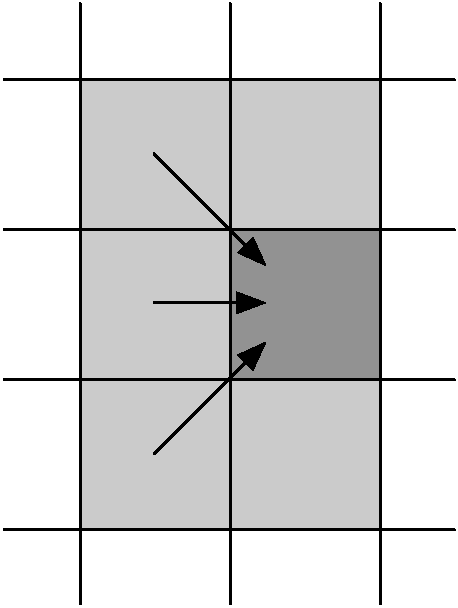
\includegraphics[width=.18\textwidth]{HiStencils/heat_transfer}
    \caption{Stencil shape for heat transfer simulation}
    \label{fig:stencilShape}
    \vspace{-.5em}
  \end{centering}
\end{figure}

Many stencil applications apply a stencil multiple times for a fixed number of iterations, or until a certain condition is met.
For example, to iterate the heat transfer simulation for one hundred steps, we specify the number of iterations to perform when executing the skeleton (line 10).
In the future, we plan to allow the user to specify a custom function which checks a condition to stop the iterations.

The MapOverlap skeleton can be configured to handle out-of-bounds accesses by returning the nearest valid value of the input matrix.
Another distinction can be made regarding iterations and sequences of stencil operations:
using elements of the \textbf{initial}, user-provided input matrix or using elements of the \textbf{current} step's input matrix, which already was updated during earlier stencil operations.
The Stencil skeleton can be configured to handle out-of-bounds accesses in both ways, thus offering three possible ways, including the neutral value. 
For each of them, there is an own kernel function, loading appropriate elements into local memory. 

\paragraph{The Stencil Skeleton}

\paragraph{Sequence of Stencil Operations}
Many real-world applications perform different stencil operations in a sequence.
Let us consider the popular \emph{Canny algorithm} which is used for detecting edges in images.
For the sake of simplicity we consider a simplified version, which applies the following stencil operations in a sequence:
first, a noise reduction operation is applied, e.g., a Gaussian filter;
second, an edge detection operator like the Sobel filter is applied;
third, the so-called non-maximum suppression is performed, where all pixels in the image are colored black except pixels being a local maximum;
finally, a threshold operation is applied to produce the final result.
A more complex version of the algorithm performs the edge tracking by hysteresis, as an additional step.
This results in detecting some weaker edges, but even without this
additional step the algorithm usually achieves good results.

In SkelCL, each single step of the Canny algorithm can be expressed using the Stencil skeleton.
The last step, threshold operation, does not need access to neighboring elements, as the user threshold function only checks the value of the current pixel.
Therefore, this step can be expressed using SkelCL's simpler Map skeleton.
The Stencil skeleton's implementation automatically uses the simpler Map skeleton's implementation when the user specifies a stencil shape which extents are $0$ in all directions.

\begin{lstlisting}[%
  caption={Structure of the Canny algorithm as implemented with a sequence of skeletons.},%
  float=tbp,%
  label={lst:canny01}]
Stencil<Pixel(Pixel)> gauss(...);
Stencil<Pixel(Pixel)> sobel(...);
Stencil<Pixel(Pixel)> nms(...);
Stencil<Pixel(Pixel)> threshold(...);

StencilSequence<Pixel(Pixel)> canny(
  gauss, sobel, nms, threshold);

output = canny(1, input);
\end{lstlisting}

To implement the Canny algorithm in SkelCL, the single steps can be combined as shown in Listing~\ref{lst:canny01}.
The individual steps are defined in lines 1--4 and then combined to a sequence of stencils in line 6 and 7.
During execution (line 9), the stencil operation are performed in the order which is specified when creating the \emph{StencilSequence} object.

\paragraph{Implementation}
In order to achieve high performance, our implementations of both the MapOverlap and the Stencil skeleton use the GPU's fast local memory.
Both implementations perform the same basic steps on the GPU:
first, the data is loaded from the global memory into the local memory;
then, the user-defined function is called for every data element by passing a pointer to the element's location in the local memory;
finally, the result of the user-defined function is copied back into the global memory.

Although both implementations perform the same basic steps, different strategies are implemented for loading the data from the global into the local memory.

\begin{figure}
  \begin{centering}
    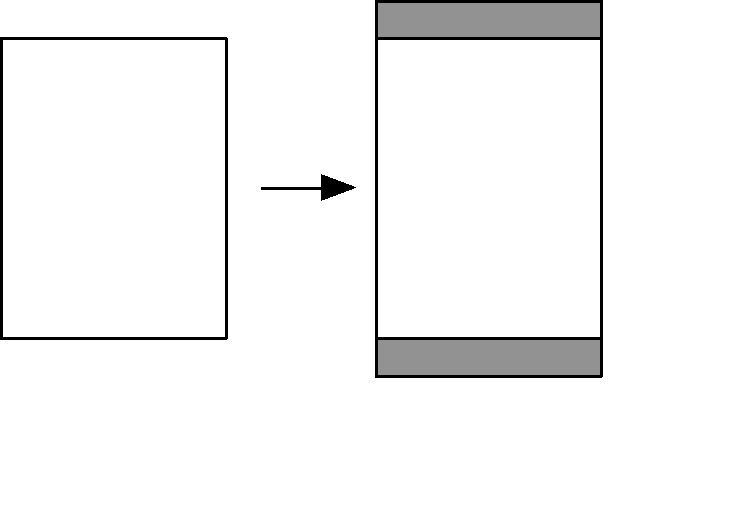
\includegraphics[width=.29\textwidth]{HiStencils/map_overlap}
    \caption{The MapOverlap skeleton prepares a matrix by copying data on the top and bottom.}
    \label{fig:preparation}
    \vspace{-.5em}
  \end{centering}
\end{figure}

The MapOverlap skeleton prepares the input matrix on the CPU before uploading it to the GPU:
padding elements are appended; they are used to avoid out-of-bounds memory accesses to the top and bottom of the input matrix, as shown in Figure~\ref{fig:preparation}.
This slightly enlarges the input matrix, but it reduces branching on the GPU due to avoiding some out-of-bound checks.
In SkelCL a matrix is stored row-wise in memory on the CPU and GPU, therefore, it would be complex and costly to add padding elements on the left and right of the matrix.
To avoid out-of-bound accesses for these regions, the boundary checks are performed on the GPU.

The Stencil skeleton has to use a different strategy in order to enable the usage of different padding modes and stencil shapes when using several Stencil skeletons in a sequence.
As an example, consider two stencil shapes in a sequence where the first shape defines a neutral element $0$ and the second defines a neutral element $1$.
This cannot be implemented using MapOverlap's implementation strategy.
Therefore, Stencil does not append padding elements on the CPU, but rather manages all out-of-bounds accesses on the GPU, which slightly increases branching.

\section{Targeting Multi-GPU Systems (HiStencils)}
\label{sec:multi_gpu}
The implicit and automatic support of systems with multiple OpenCL devices is one of the key features of SkelCL.
By using distributions, SkelCL completely liberates the user from error-prone and low-level explicit programming of data (re)distributions on multiple GPUs. 

The MapOverlap skeleton uses the overlap distribution with \textit{border regions} in which the elements calculated by a neighboring device are located.
When it comes to iteratively executing a skeleton, data has to be transferred among devices between iteration steps, in order to ensure that data for the next iteration step is up-to-date.
As the MapOverlap skeleton does not explicitly support iterations, its implementation is not able to exchange data between devices besides a full down- and upload of the matrix.
In addition, data exchange has to be performed after each iteration.
We can enlarge the number of elements in the border regions and perform multiple iteration steps on each device before exchanging data.
However, this introduces redundant computations, such that a trade-off between data exchange and redundant computations has to be found.
 
For the Stencil skeleton, the user can specify the number of iterations between \textit{device synchronisations}, where all border regions are updated with elements from the corresponding inner border regions of the neighboring device.
The border regions are sized by default in such a way that the specified number of iterations can be performed without leading to incorrect results.
However, there may be cases in which a different number of iterations between device synchronizations may result in better performance.
Therefore, Stencil offers the user the possibility to specify that number.
Please note that the implementation of the Stencil skeleton only exchanges elements from the border region and does not perform a full down- and upload of the matrix, as the MapOverlap skeleton does.

Figure \ref{fig:syncDevices} shows the device synchronization.
Only the appropriate elements in the inner border region are downloaded and stored as \texttt{std::vector}s in a \texttt{std::vector}.
Within the outer vector, the inner vectors are swapped pair-wise on the host, so that the inner border regions can be uploaded in order to replace the out-of-date border regions.

For the first iteration after a device synchronization, there are as many work-items on the GPU active as there are total elements on the device.
As the first and last rows of the border regions become invalid within an iteration, the corresponding work-items become inactive in the following iteration step.
This is done by using an offset and by reducing the number of total work-items when launching the OpenCL kernel.
The Stencil's four kernel functions (one for each out-of-bounds handling mode and one for the adapted Map skeleton) can be used for both single- and multi-GPU systems.
 
\begin{figure}[tb]
	\centering
	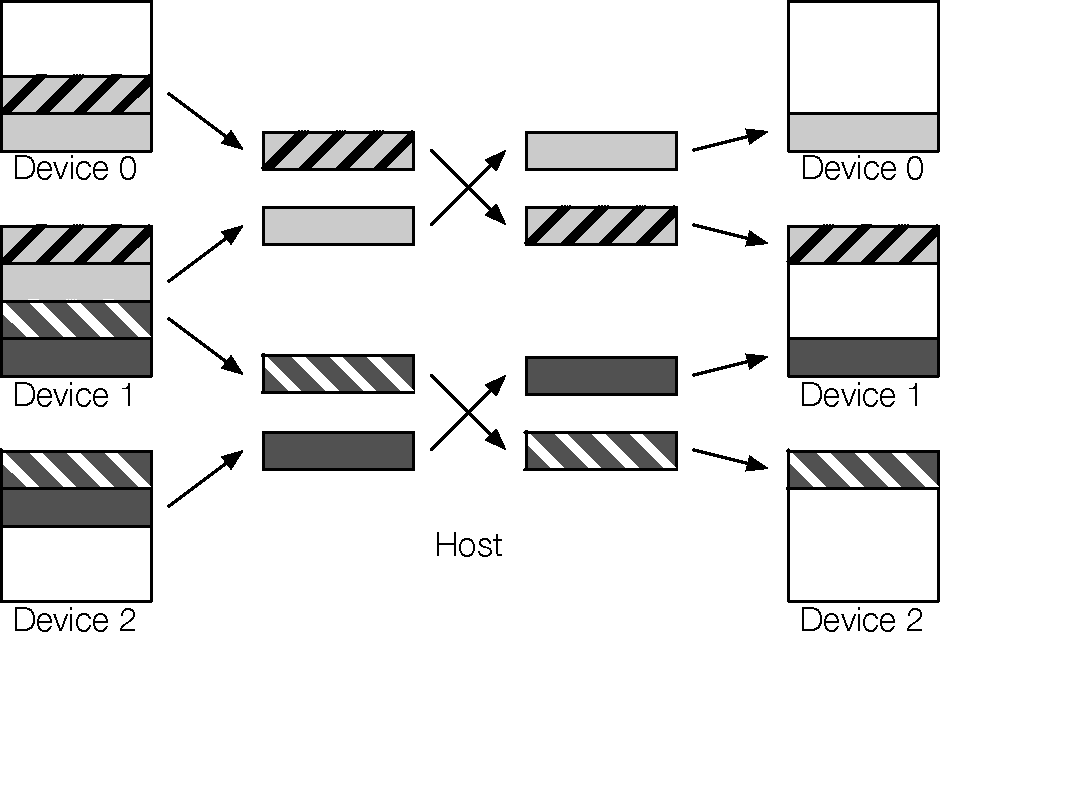
\includegraphics[width=\columnwidth]{HiStencils/data_exchange}
	\caption{\small Device synchronization for three devices. Equally patterned and colored chunks represent the border regions and their matching inner border region. After the download of the appropriate inner border regions, they are swapped pair-wise on the host. Then the inner border regions are uploaded in order to replace the out-of-date border regions.}
	\label{fig:syncDevices}
  \vspace{1em}
\end{figure} 
\from{HiStencils end}

